 \documentclass[conference]{IEEEtran}
\IEEEoverridecommandlockouts
% The preceding line is only needed to identify funding in the first footnote. If that is unneeded, please comment it out.
\usepackage{cite}
\usepackage{amsmath,amssymb,amsfonts}
\usepackage{algorithmic}
\usepackage{graphicx}
\usepackage{textcomp}
\usepackage{xcolor}
\usepackage{multirow}
\usepackage{caption}
\usepackage{booktabs}

\usepackage{amsthm}
\usepackage{amssymb}
\usepackage{makecell}
\usepackage{enumitem}
\usepackage{dblfloatfix}

% Define the claim environment in the preamble
\newtheorem{claim}{Claim}
\newcommand{\draft}[1]{{\color{black}{#1}}}

\newcommand\JI[1]{\textcolor{red}{JI: #1}}
% Define the corollary environment, sharing the counter with 'claim'
\newtheorem{corollary}{Corollary}[claim]

\def\BibTeX{{\rm B\kern-.05em{\sc i\kern-.025em b}\kern-.08em
    T\kern-.1667em\lower.7ex\hbox{E}\kern-.125emX}}

\author{Jacob Carter, Vaishnav Ramesh, Md Jahidul Islam, and Sanjeev J. Koppal\textsuperscript{\textdagger}% <-this % stops a space
% \thanks{*This work was not supported by any organization}% <-this % stops a space
\thanks{All authors are affiliated with the Dept.~of Electrical and Computer Engineering, University of Florida, Gainesville, FL 32611, USA.
E-mail: carterjacob@ufl.edu (corresponding author).}
\thanks{\textsuperscript{\textdagger}
Dr.~Sanjeev~J.~Koppal holds concurrent appointments as an Associate Professor of ECE at the University of Florida and as an Amazon Scholar at Amazon Robotics. This project was performed at the University of Florida and is not associated with Amazon Robotics.}% <-this % stops an unwanted space
%
}
\begin{document}

\title{\vspace{5mm}Anchor Points for Monocular Depth Estimation Under Severe Rolling Shutter Ego-motion%
% \vspace{-15mm}
}
%\title{Anchor Points for Monocular Depth Estimation Under Severe Rolling Shutter Ego-motion}
%\title{Monocular Depth from Rolling Shutter Distortions Induced by Ego-motion}



%author{\IEEEauthorblockN{1\textsuperscript{st} Jacob Carter}
% \IEEEauthorblockA{\textit{Electrical and Computer Engineering} \\
% \textit{University of Florida}\\
% Gainesville, United States \\
% carterjacob@ufl.edu}
% \and
% \IEEEauthorblockN{2\textsuperscript{th} Sanjeev J. Koppal}
% \IEEEauthorblockA{\textit{Electrical and Computer Engineering} \\
% \textit{University of Florida}\\
% Gainesville, United States \\
% sjkoppal@ece.ufl.edu}
% }

% \twocolumn[{%
% \renewcommand\twocolumn[1][]{#1}%
% \maketitle
%  \IEEEpeerreviewmaketitle
% \begin{center}
%     
% \centering
%     % Input Image
%     \begin{minipage}{0.03\textwidth} % Narrow column for row label
%         \raggedleft
%         \rotatebox{90}{\text{Input Image}} % Vertical label for the first row
%     \end{minipage}
%     \begin{minipage}{0.12\textwidth}
%         \vspace{0.03cm}
%         \centering
%         
\includegraphics[width=\textwidth]{Collocated_Collage/input/frame344.png}
%     \end{minipage}
%     \begin{minipage}{0.12\textwidth}
%         \vspace{0.03cm}
%         \centering
%         
\includegraphics[width=\textwidth]{Collocated_Collage/input/frame44.png}
%     \end{minipage}
%     \begin{minipage}{0.12\textwidth}
%         \vspace{0.03cm}
%         \centering
%         
\includegraphics[width=\textwidth]{Collocated_Collage/input/frame129.png}
%     \end{minipage}
%     \begin{minipage}{0.12\textwidth}
%         \vspace{0.03cm}
%         \centering
%         
\includegraphics[width=\textwidth]{Collocated_Collage/10-20-vis/input/frame205.png}
%     \end{minipage}
%     \begin{minipage}{0.12\textwidth}
%         \vspace{0.03cm}
%         \centering
%         
\includegraphics[width=\textwidth]{Collocated_Collage/input/frame338.png}
%     \end{minipage}
%     \begin{minipage}{0.12\textwidth}
%         \vspace{0.03cm}
%         \centering
%         
\includegraphics[width=\textwidth]{Collocated_Collage/input/frame79.png}
%     \end{minipage}
%     \begin{minipage}{0.12\textwidth}
%         \vspace{0.03cm}
%         \centering
%         
\includegraphics[width=\textwidth]{Collocated_Collage/input/frame13.png}
%     \end{minipage}
%     \hspace{0.03\textwidth}
    


%     \begin{minipage}{0.03\textwidth} % Narrow column for row label
%         \raggedleft
%         \rotatebox{90}{\text{Ours}} % Vertical label for the first row
%     \end{minipage}
%       \begin{minipage}{0.12\textwidth}
%         \vspace{0.03cm}
%         \centering
%         
\includegraphics[width=\textwidth]{Collocated_Collage/output_bw_color/frame344.png}
%     \end{minipage}
%     \begin{minipage}{0.12\textwidth}
%         % \vspace{0.03cm}
%         \centering
%         
\includegraphics[width=\textwidth]{Collocated_Collage/output_bw_color/frame44.png}
%     \end{minipage}
%     \begin{minipage}{0.12\textwidth}
%         \vspace{0.03cm}
%         \centering
%         
\includegraphics[width=\textwidth]{Collocated_Collage/output_bw_color/frame129.png}
%     \end{minipage}
%     \begin{minipage}{0.12\textwidth}
%         \vspace{0.03cm}
%         \centering
%         
\includegraphics[width=\textwidth]{Collocated_Collage/10-20-vis/output/frame205.png}
%     \end{minipage}
%     \begin{minipage}{0.12\textwidth}
%         \vspace{0.03cm}
%         \centering
%         
\includegraphics[width=\textwidth]{Collocated_Collage/output_bw_color/frame338.png}
%     \end{minipage}
%     \begin{minipage}{0.12\textwidth}
%         \vspace{0.03cm}
%         \centering
%         
\includegraphics[width=\textwidth]{Collocated_Collage/output_bw_color/frame79.png}
%     \end{minipage}
%     \begin{minipage}{0.12\textwidth}
%         \vspace{0.03cm}
%         \centering
%         
\includegraphics[width=\textwidth]{Collocated_Collage/output_bw_color/frame13.png}
%     \end{minipage}
%     \hspace{0.03\textwidth}
    
%     \begin{minipage}{0.03\textwidth} % Narrow column for row label
%         \raggedleft
%         \rotatebox{90}{\text{Ground Truth}} % Vertical label for the first row
%       \end{minipage}
%       \begin{minipage}{0.12\textwidth}
%         \vspace{0.03cm}
%         \centering
%         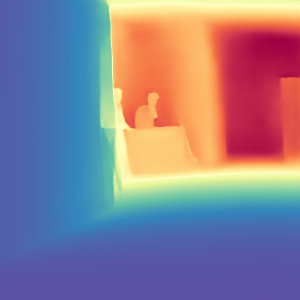
\includegraphics[width=\textwidth]{Collocated_Collage/gt_depth_color/frame344.png}
%     \end{minipage}
%     \begin{minipage}{0.12\textwidth}
%         % \vspace{0.03cm}
%         \centering
%         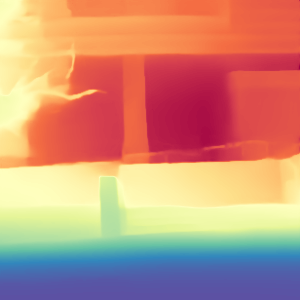
\includegraphics[width=\textwidth]{Collocated_Collage/gt_depth_color/frame44.png}
%     \end{minipage}
%     \begin{minipage}{0.12\textwidth}
%         \vspace{0.03cm}
%         \centering
%         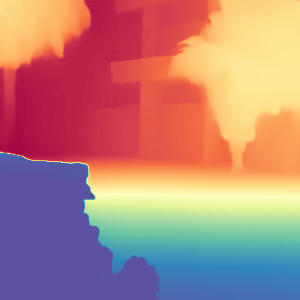
\includegraphics[width=\textwidth]{Collocated_Collage/gt_depth_color/frame129.png}
%     \end{minipage}
%     \begin{minipage}{0.12\textwidth}
%         \vspace{0.03cm}
%         \centering
%         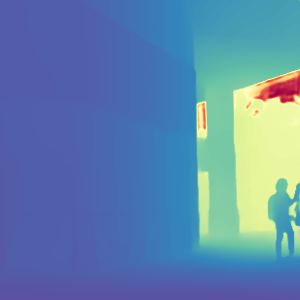
\includegraphics[width=\textwidth]{Collocated_Collage/10-20-vis/gt/frame205.png}
%     \end{minipage}
%     \begin{minipage}{0.12\textwidth}
%         \vspace{0.03cm}
%         \centering
%         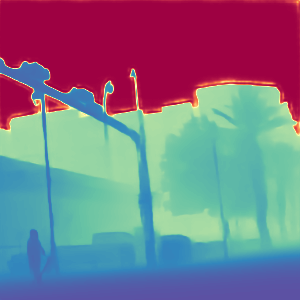
\includegraphics[width=\textwidth]{Collocated_Collage/gt_depth_color/frame338.png}
%     \end{minipage}
%     \begin{minipage}{0.12\textwidth}
%         \vspace{0.03cm}
%         \centering
%         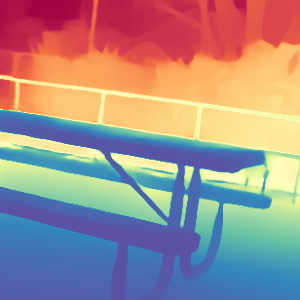
\includegraphics[width=\textwidth]{Collocated_Collage/gt_depth_color/frame79.png}
%     \end{minipage}
%     \begin{minipage}{0.12\textwidth}
%         \vspace{0.03cm}
%         \centering
%         
\includegraphics[width=\textwidth]{Collocated_Collage/gt_depth_color/frame13.png}
%     \end{minipage}
%     \hspace{0.03\textwidth}
%\vspace{-5mm}
    \centering
    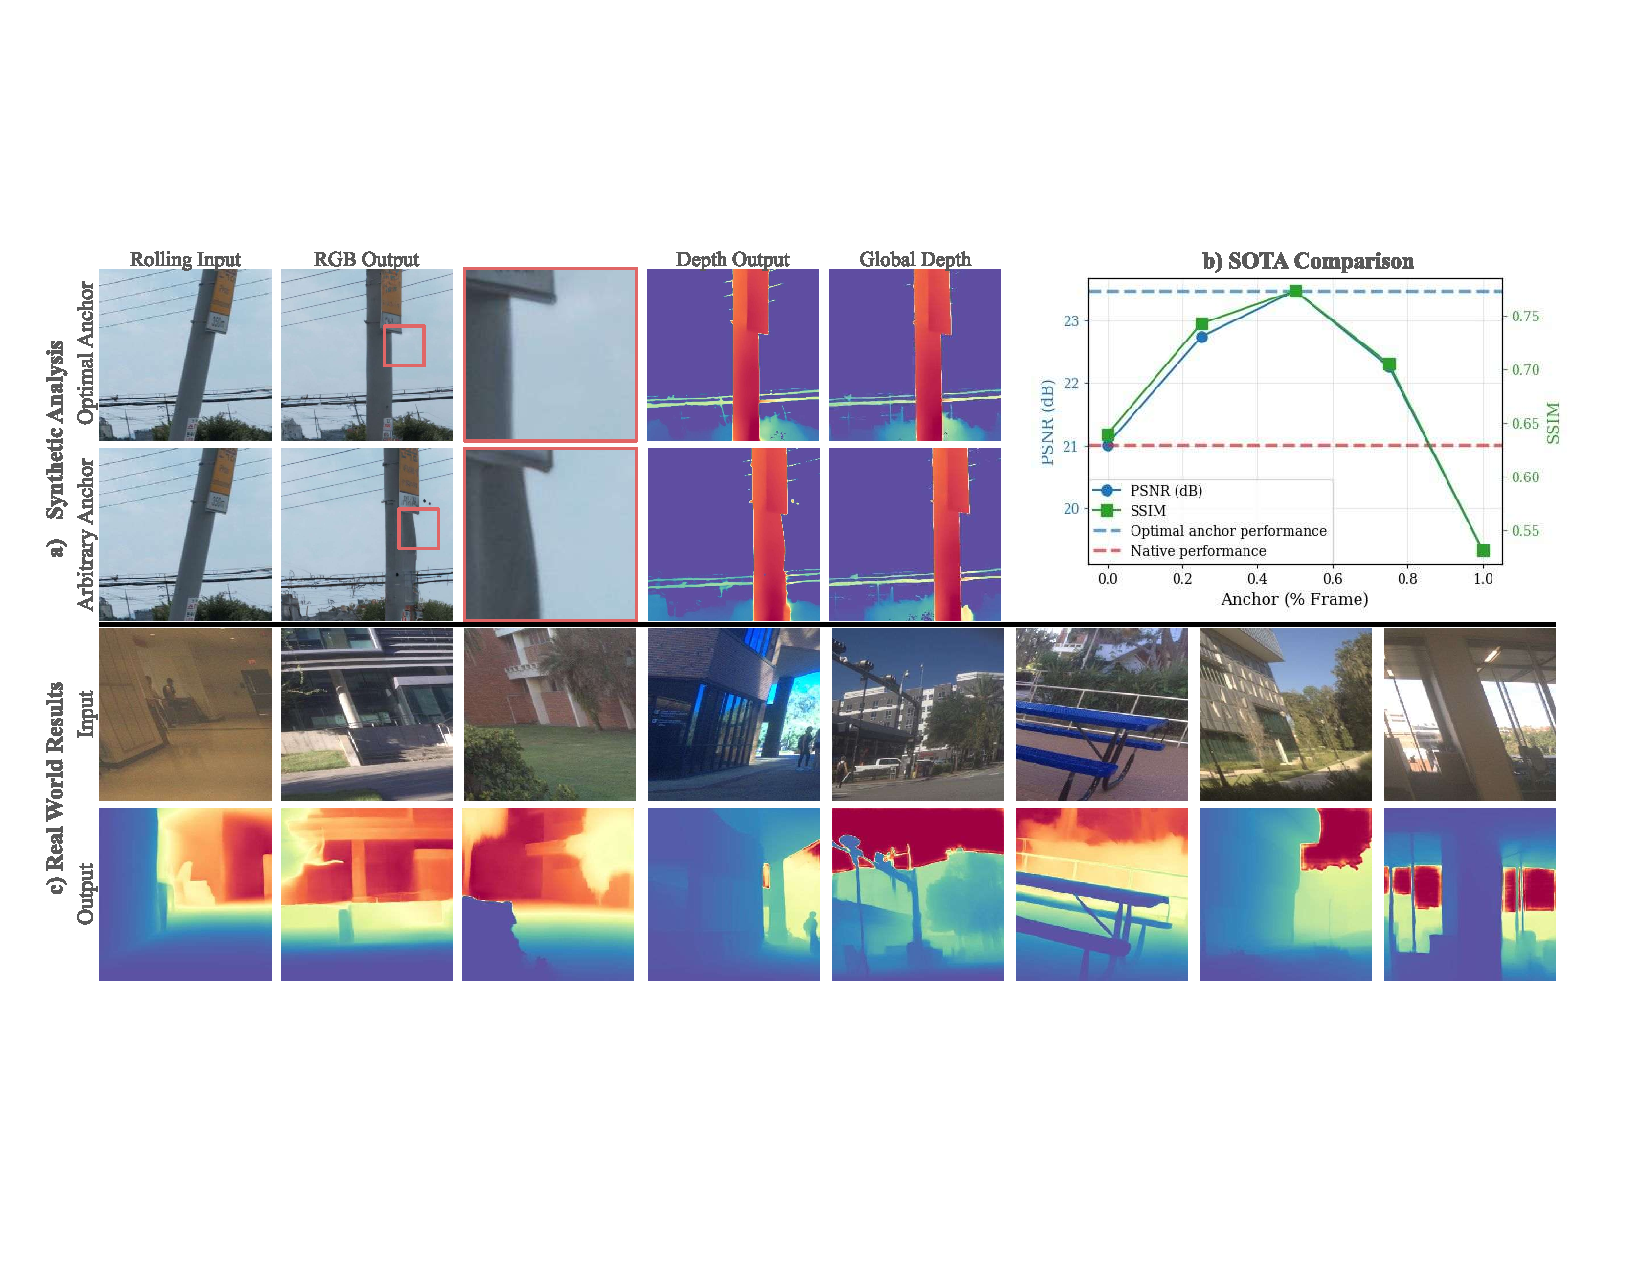
\includegraphics[width=0.95\linewidth,trim={.7cm 4.5cm 1cm 4.2cm},clip]{Figures/Rolling Shutter.pdf}%
    \vspace{-4mm}
    \captionof{figure}{
    \textbf{Anchor point formulation for rolling shutter correction}:
    \textbf{a)} We introduce the concept of an \emph{anchor point}, which defines the temporal reference used to align rolling shutter observations during correction.
    \textbf{b)} Quantitative analysis on a SOTA rolling shutter correction method~\cite{RS-Diffusion} shows that performance varies systematically with anchor-point selection, providing a significant metric boost around the proposed optimal anchor when compared to native implementation. This modification is \textbf{one line of code}, requiring no retraining of the model.
    \textbf{c)} We introduce visual foundation models to rolling shutter correction, providing geometrically consistent monocular depth from large rolling shutter distortions.
    }
    \label{fig:teaser_results}

% \end{center}%
% }]


\maketitle 

\begin{figure*}
    
% \centering
%     % Input Image
%     \begin{minipage}{0.03\textwidth} % Narrow column for row label
%         \raggedleft
%         \rotatebox{90}{\text{Input Image}} % Vertical label for the first row
%     \end{minipage}
%     \begin{minipage}{0.12\textwidth}
%         \vspace{0.03cm}
%         \centering
%         
\includegraphics[width=\textwidth]{Collocated_Collage/input/frame344.png}
%     \end{minipage}
%     \begin{minipage}{0.12\textwidth}
%         \vspace{0.03cm}
%         \centering
%         
\includegraphics[width=\textwidth]{Collocated_Collage/input/frame44.png}
%     \end{minipage}
%     \begin{minipage}{0.12\textwidth}
%         \vspace{0.03cm}
%         \centering
%         
\includegraphics[width=\textwidth]{Collocated_Collage/input/frame129.png}
%     \end{minipage}
%     \begin{minipage}{0.12\textwidth}
%         \vspace{0.03cm}
%         \centering
%         
\includegraphics[width=\textwidth]{Collocated_Collage/10-20-vis/input/frame205.png}
%     \end{minipage}
%     \begin{minipage}{0.12\textwidth}
%         \vspace{0.03cm}
%         \centering
%         
\includegraphics[width=\textwidth]{Collocated_Collage/input/frame338.png}
%     \end{minipage}
%     \begin{minipage}{0.12\textwidth}
%         \vspace{0.03cm}
%         \centering
%         
\includegraphics[width=\textwidth]{Collocated_Collage/input/frame79.png}
%     \end{minipage}
%     \begin{minipage}{0.12\textwidth}
%         \vspace{0.03cm}
%         \centering
%         
\includegraphics[width=\textwidth]{Collocated_Collage/input/frame13.png}
%     \end{minipage}
%     \hspace{0.03\textwidth}
    


%     \begin{minipage}{0.03\textwidth} % Narrow column for row label
%         \raggedleft
%         \rotatebox{90}{\text{Ours}} % Vertical label for the first row
%     \end{minipage}
%       \begin{minipage}{0.12\textwidth}
%         \vspace{0.03cm}
%         \centering
%         
\includegraphics[width=\textwidth]{Collocated_Collage/output_bw_color/frame344.png}
%     \end{minipage}
%     \begin{minipage}{0.12\textwidth}
%         % \vspace{0.03cm}
%         \centering
%         
\includegraphics[width=\textwidth]{Collocated_Collage/output_bw_color/frame44.png}
%     \end{minipage}
%     \begin{minipage}{0.12\textwidth}
%         \vspace{0.03cm}
%         \centering
%         
\includegraphics[width=\textwidth]{Collocated_Collage/output_bw_color/frame129.png}
%     \end{minipage}
%     \begin{minipage}{0.12\textwidth}
%         \vspace{0.03cm}
%         \centering
%         
\includegraphics[width=\textwidth]{Collocated_Collage/10-20-vis/output/frame205.png}
%     \end{minipage}
%     \begin{minipage}{0.12\textwidth}
%         \vspace{0.03cm}
%         \centering
%         
\includegraphics[width=\textwidth]{Collocated_Collage/output_bw_color/frame338.png}
%     \end{minipage}
%     \begin{minipage}{0.12\textwidth}
%         \vspace{0.03cm}
%         \centering
%         
\includegraphics[width=\textwidth]{Collocated_Collage/output_bw_color/frame79.png}
%     \end{minipage}
%     \begin{minipage}{0.12\textwidth}
%         \vspace{0.03cm}
%         \centering
%         
\includegraphics[width=\textwidth]{Collocated_Collage/output_bw_color/frame13.png}
%     \end{minipage}
%     \hspace{0.03\textwidth}
    
%     \begin{minipage}{0.03\textwidth} % Narrow column for row label
%         \raggedleft
%         \rotatebox{90}{\text{Ground Truth}} % Vertical label for the first row
%       \end{minipage}
%       \begin{minipage}{0.12\textwidth}
%         \vspace{0.03cm}
%         \centering
%         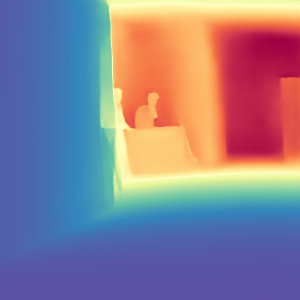
\includegraphics[width=\textwidth]{Collocated_Collage/gt_depth_color/frame344.png}
%     \end{minipage}
%     \begin{minipage}{0.12\textwidth}
%         % \vspace{0.03cm}
%         \centering
%         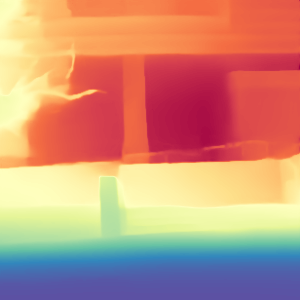
\includegraphics[width=\textwidth]{Collocated_Collage/gt_depth_color/frame44.png}
%     \end{minipage}
%     \begin{minipage}{0.12\textwidth}
%         \vspace{0.03cm}
%         \centering
%         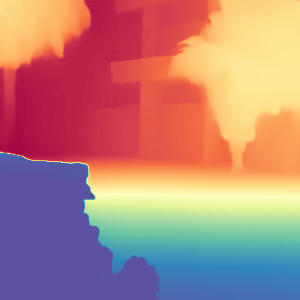
\includegraphics[width=\textwidth]{Collocated_Collage/gt_depth_color/frame129.png}
%     \end{minipage}
%     \begin{minipage}{0.12\textwidth}
%         \vspace{0.03cm}
%         \centering
%         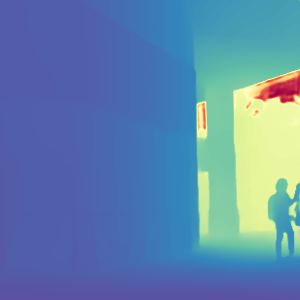
\includegraphics[width=\textwidth]{Collocated_Collage/10-20-vis/gt/frame205.png}
%     \end{minipage}
%     \begin{minipage}{0.12\textwidth}
%         \vspace{0.03cm}
%         \centering
%         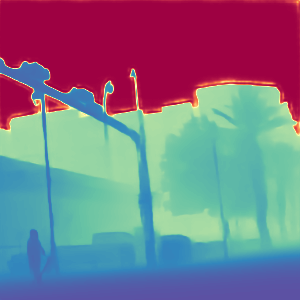
\includegraphics[width=\textwidth]{Collocated_Collage/gt_depth_color/frame338.png}
%     \end{minipage}
%     \begin{minipage}{0.12\textwidth}
%         \vspace{0.03cm}
%         \centering
%         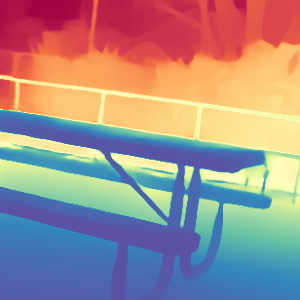
\includegraphics[width=\textwidth]{Collocated_Collage/gt_depth_color/frame79.png}
%     \end{minipage}
%     \begin{minipage}{0.12\textwidth}
%         \vspace{0.03cm}
%         \centering
%         
\includegraphics[width=\textwidth]{Collocated_Collage/gt_depth_color/frame13.png}
%     \end{minipage}
%     \hspace{0.03\textwidth}
%\vspace{-5mm}
    \centering
    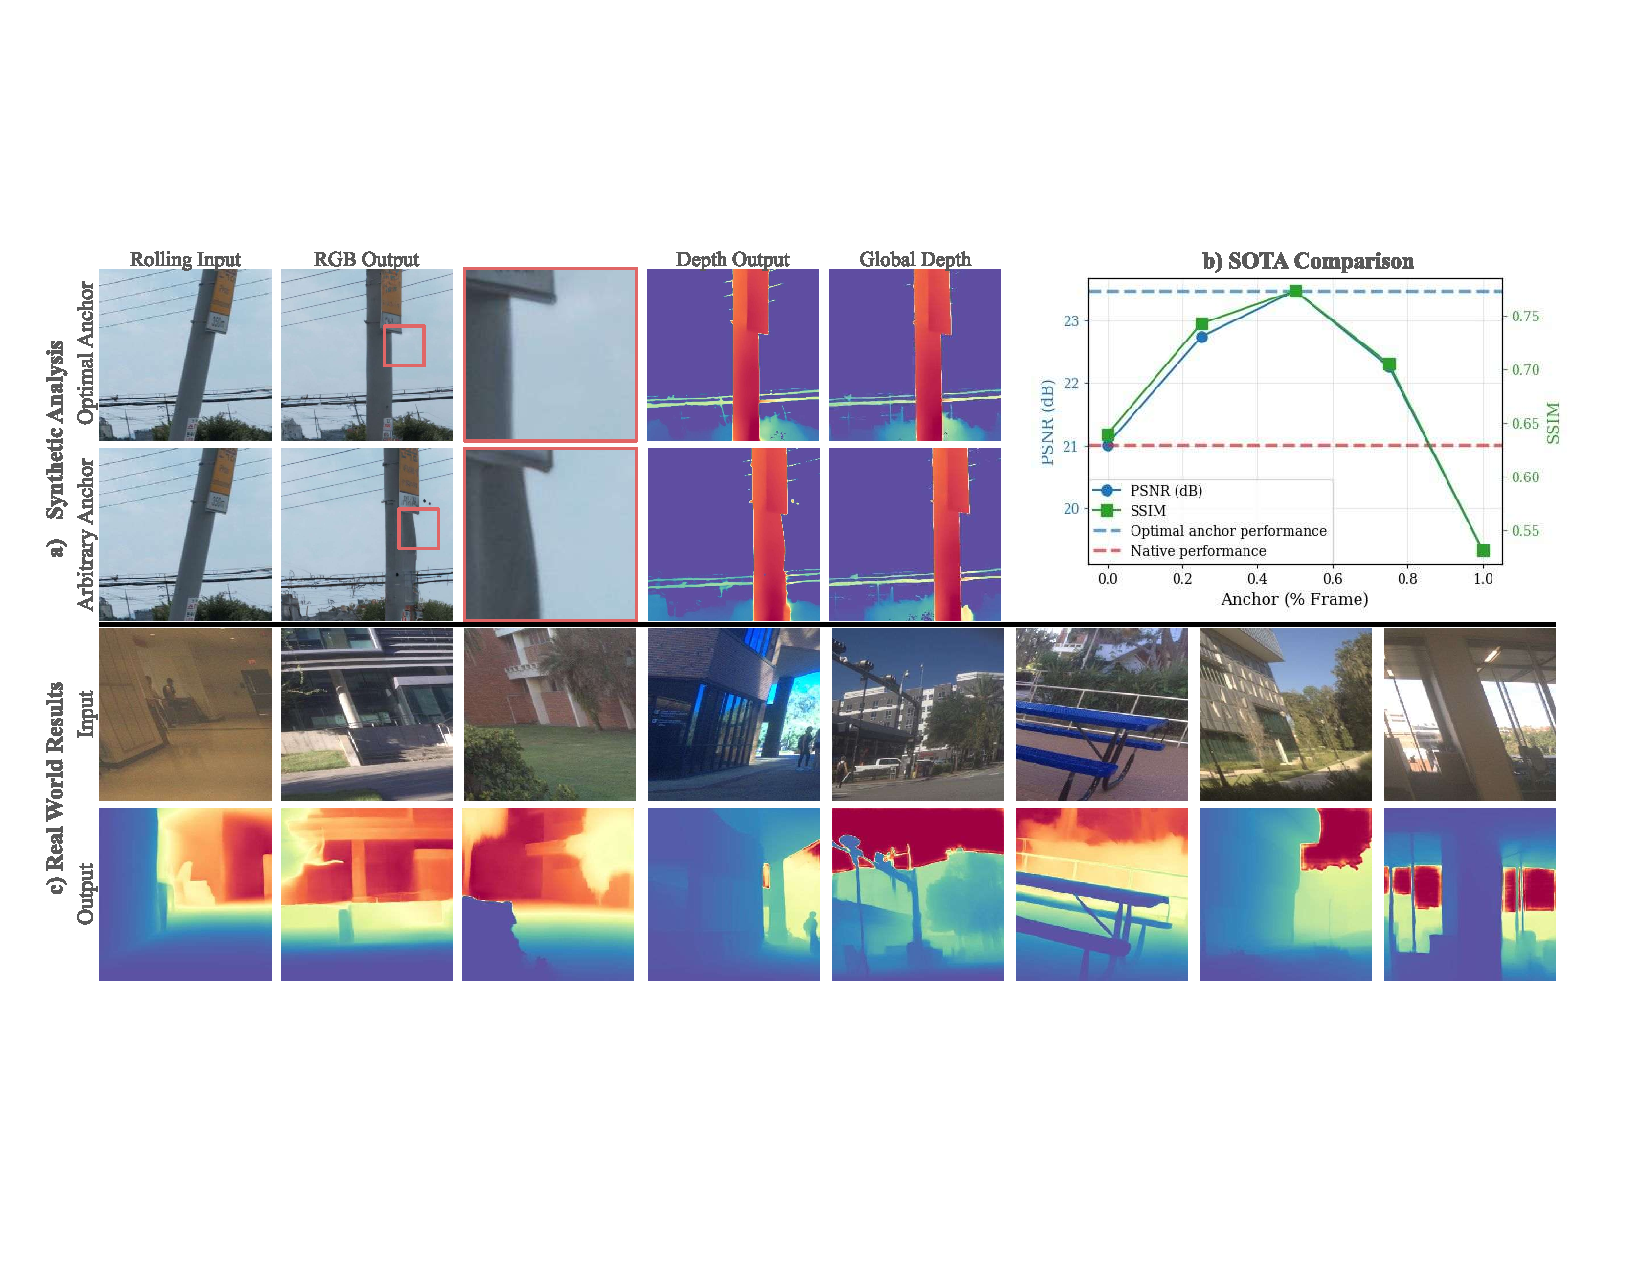
\includegraphics[width=0.95\linewidth,trim={.7cm 4.5cm 1cm 4.2cm},clip]{Figures/Rolling Shutter.pdf}%
    \vspace{-4mm}
    \captionof{figure}{
    \textbf{Anchor point formulation for rolling shutter correction}:
    \textbf{a)} We introduce the concept of an \emph{anchor point}, which defines the temporal reference used to align rolling shutter observations during correction.
    \textbf{b)} Quantitative analysis on a SOTA rolling shutter correction method~\cite{RS-Diffusion} shows that performance varies systematically with anchor-point selection, providing a significant metric boost around the proposed optimal anchor when compared to native implementation. This modification is \textbf{one line of code}, requiring no retraining of the model.
    \textbf{c)} We introduce visual foundation models to rolling shutter correction, providing geometrically consistent monocular depth from large rolling shutter distortions.
    }
    \label{fig:teaser_results}

\end{figure*}

\begin{abstract}
Rolling shutter (RS) cameras are widely deployed in robotic systems due to their low cost and power efficiency. However, robot ego-motion induces significant RS distortions that degrade geometric consistency and severely challenge visual perception. In this work, we address monocular depth estimation under large rolling shutter distortions caused by ego-motion. We introduce the concept of an anchor point, which establishes a consistent temporal and geometric reference between rolling shutter and global shutter observations. This formulation enables principled adaptation and fine-tuning of deep foundation models for depth estimation under RS distortions. To systematically evaluate the problem, we present a new rolling shutter dataset featuring large motion-induced geometric distortions representative of mobile robotic tasks. Our experimental analysis shows that anchor point selection is a primary factor governing depth accuracy under RS effects. We further characterize anchor configurations for RS-GS data capture and identify stable regimes that yield accurate depth estimates. Using a representative two-stage depth estimation pipeline, we conduct extensive ablation studies demonstrating that anchor-based modeling significantly improves performance, outperforming recent RS correction baselines under strong ego-motion. Finally, we validate our approach on a legged robot platform, demonstrating robust monocular depth estimation in the presence of substantial rolling shutter distortions in under 400 ms.
%In this paper, we focus on monocular depth estimation, a crucial robot perception task, in the face of large RS distortions. We introduce the concept of an \textit{anchor point}, which defines a consistent temporal and geometric reference between rolling shutter and global shutter observations and enables effective fine-tuning of deep foundational models under RS distortions. We also introduce a new RS dataset to evaluate our method with large geometric distortions that are common in mobile robot vision tasks. Our experiments show that the choice of temporal anchor point enables high performance on our new dataset, where egocentric motions amplify RS distortions. We analyze anchor point selection for RS-GS data capture and identify configurations that yield stable and accurate depth estimates. Using a representative two-stage depth estimation pipeline, we show through extensive ablations that anchor point choice and dataset design are primary drivers of performance, outperforming recent RS correction baselines under large ego-motion. We also show a legged robot experiment demonstrating near real-time performance of the monocular depth estimation.
\end{abstract}
% \begin{figure}
%     \centering
%     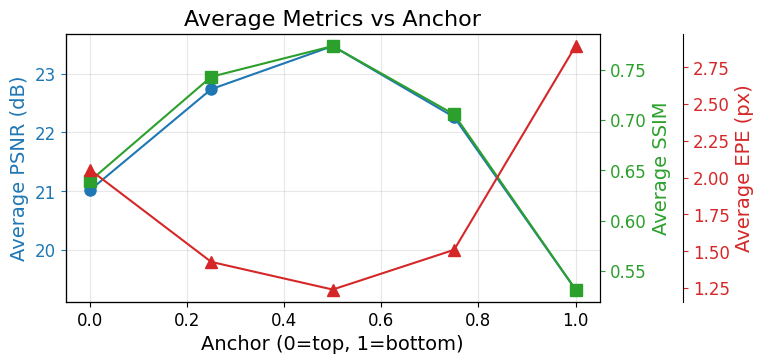
\includegraphics[width=\linewidth]{Figures/rs-diff.png}%
%     \vspace{-2mm}
%     \caption{Demonstration of the proposed \textit{anchor point} formulation using a representative rolling shutter depth framework~\cite{RS-Diffusion}. Our theory predicts an optimal anchor point at $N/2$. By modifying only the anchor-point selection, while keeping the original implementation and pretrained weights unchanged, we observe substantial performance improvements \textit{without retraining}. The plotted results confirm that performance peaks near the theoretically predicted anchor location. \JI{What is N? - revise and address}
%     %As a demonstration of our \textit{anchor point} idea, consider the state-of-the-art paper RS Diffusion \cite{RS-Diffusion}. Our theory predicts an anchor point of $\frac{N}{2}$, which the authors of \cite{RS-Diffusion} do not use -- instead, they use an anchor point of $0$ (most prior RS researchers use an arbitrary anchor point by default). By using \textit{their code} and \textit{their dataset}, and by changing only a \textit{single line of code} to vary the anchor point, we can achieve significantly better results \textit{with no retraining}. The graphs show the optimal value is at our predicted anchor point $\frac{N}{2}$.
%     } 
%     \label{fig:rs-diff_comp}
%     \vspace{-5mm}
% \end{figure}


\section{Introduction}

Rolling shutter (RS) effects arise from row-by-row image readout, causing each scanline to be captured at a different time rather than simultaneously as in global shutter (GS) imaging. In dynamic scenes, this temporal offset induces complex geometric distortions that depend on both camera ego-motion and scene dynamics. RS cameras remain ubiquitous in modern robotic systems because they are compact, power-efficient, and cost-effective compared to global shutter alternatives\cite{4549748}. 
% While prior work on rolling shutter correction (RSC) has shown progress for mild or structured distortions, performance often degrades under large, nonlinear RS effects frequently encountered in real robotic deployments\ref{fig:collocated_results}. As a result, reliable monocular depth estimation from single-view RS imagery remains challenging. 

Prior work addresses RS correction using geometric and learning-based methods. Rolling-shutter-aware pose estimation has also been explored in robotics to mitigate downstream effects.
Despite these advances, existing methods struggle with single-frame images under large distortions, often assuming mild motion, requiring extra sensors, or relying on temporal context. Moreover, learning-based methods fix a temporal reference implicitly, yet the impact of this choice on geometric consistency and depth prediction remains underexplored. Due to this lack of exploration, reliable monocular depth estimation from large RS distortions remains a challenge.

% \JI{It is great that the first paragraph mentions "what is the problem and why is this important". Although needs citations. The second paragraph is missing where you talk about "what other people have done and what specific challenges remain". The second paragraph is missing}


% "what are you proposing"
% A central component of our approach is the \textbf{anchor point}, a temporal reference that specifies which GS frame an RS image corresponds to. \textit{While the idea is simple, many modern RSC algorithms don't optimize their selection of anchor point \cite{RS-Diffusion}, \cite{DeepUnrollNet}}. This change alone yields a significant performance improvement without retraining (Fig.~\ref{fig:teaser_results}). Through this and additional analysis, we show that anchor point selection strongly influences correction quality and downstream depth estimation, particularly under severe RS distortions. We analyze anchor point configurations systematically and identify selections that yield stable and geometrically consistent reconstructions.
% %\JI{I dont think you motivated your method well. Will talk more in person}

% % "how we evaluate it"
% To evaluate these effects in realistic settings, we introduce a new co-located RS-GS \textbf{dataset} designed to capture the motion profiles and imaging artifacts common in robotic systems. Using a custom beam-splitter camera rig with explicit delay control, we precisely specify anchor points during data capture, enabling fine-grained analysis of RS correction performance under large distortions. We evaluate our approach using a two-stage visual foundation pipeline that performs RSC followed by monocular depth estimation. Across synthetic and real-world benchmarks, our results demonstrate improved robustness to extreme RS distortions and large ego-motion.

%Attempt to get back real estate by fusing past two parag.
A central component of our approach is the \textbf{anchor point}, a temporal reference that specifies which GS frame a RS image is aligned to.  \draft{Existing RS correction methods implicitly select a temporal reference frame, yet the consequences of this choice have not been systematically analyzed \cite{RS-Diffusion,DeepUnrollNet}. We formalize this reference as an anchor point, derive conditions governing its optimal selection, and demonstrate experimentally that anchor-point choice is a first-order factor affecting both rolling shutter correction and downstream monocular depth estimation.} Adjusting this reference alone can yield substantial performance gains without retraining (see Fig.~\ref{fig:teaser_results}). For comprehensive evaluation, we introduce a new collocated RS–GS dataset captured with a beam-splitter rig that provides explicit control over anchor points. Using this dataset and a two-stage visual foundation pipeline for RS correction and depth estimation, we demonstrate improved robustness to large distortions and aggressive ego-motion across synthetic and real-world benchmarks.
% While conceptually simple, many modern RSC methods fix this reference implicitly and do not optimize its selection
\vspace{1mm}
\noindent
{Our contributions are as follows:}
\begin{enumerate}
    \item We introduce the concept of ``\textit{anchor point}" as a temporal reference for rolling shutter to global shutter (RS-GS) alignment, and provide a systematic analysis of its role in rolling shutter correction and monocular depth estimation under severe geometric distortions (Sect. III).

    %\item We introduce the concept of \textbf{anchor point}, a temporal reference for RS-GS alignment, and analyze its impact on rolling shutter correction and monocular depth estimation under large distortions (\figurename~ {3}).
    \item We present a new collocated RS-GS dataset with explicit anchor-point control, designed to capture realistic robotic motion with large ego-motion effects and practical imaging artifacts (Figs.~3-5).

    %We present a new co-located RS-GS dataset with explicit anchor-point control, designed to reflect realistic robotic motion and imaging artifacts (\figurename~{3, 4, 5}).
    \item We conduct extensive ablation studies across both synthetic and real-world data to quantify the influence of anchor point selection on reconstruction accuracy and depth consistency (Figs.~6-7, Tables~II-III).

    %We provide extensive ablation studies evaluating anchor point selection across synthetic and real data (\figurename~ {6, 7}, Table 2-3).
    \item We develop a two-stage foundation-model-based pipeline and demonstrate its effectiveness for rolling shutter correction and monocular depth estimation under extreme distortions and aggressive ego-motion (\figurename~8, Table~I).
    %We demonstrate the effectiveness of our approach for RS correction and monocular depth estimation under extreme distortions and large ego-motion with a two-stage foundation model pipeline (\figurename~{8}, Table~{1}).
    \item We validate the proposed system at 400\,ms end-to-end latency on a legged robot with a collocated sensor setup (\figurename~10).
    % , including live 3D reconstruction visualization
    %We demonstrate our system in near-real time (400ms latency) with a co-located system on top of a robot with reconstruction visualization (\figurename~ {10}).
\end{enumerate}

The proposed framework demonstrates promise for near-real-time RSC by mobile robots under challenging motion conditions. Its validation on a legged robot, subjected to rapid, irregular ego-motion, highlights its viability in real-world applications.



\section{Related Work}
\label{sec:related_works}

\noindent \textbf{Rolling shutter correction.}
Early single-frame approaches estimate camera motion from visual cues such as line geometry or motion blur \cite{BowsToArrows, Manhattan,MotionBlur}, while multi-frame methods rely on tracking or interpolation across image sequences to recover parametric motion models \cite{AnalysisAndCompensation, RemovingWobble,CFRS}.
Recent learning-based methods address RS correction using paired RS-GS data \cite{DeepUnrollNet,RS-Diffusion}. Diffusion-based approaches have shown promise for single-frame RS correction \cite{RS-Diffusion}, but assume moderate distortions or rely on additional sensing such as IMU measurements. In contrast, our work focuses on large RS distortions without external sensor input, emphasizing the role of temporal reference selection in downstream depth estimation.

\vspace{1mm}
\noindent \textbf{Rolling shutter in robotics.}  
Classical visual odometry (VO) and SLAM pipelines often assume global shutter imagery, leading to degraded pose and structure estimation under RS effects \cite{Hedborg2012,Meingast2005}. Continuous-time trajectory representations and rolling-shutter-aware bundle adjustment have been proposed to mitigate these effects \cite{mo2022imu,Furgale2012}, while minimal solvers for RS relative pose enable robust RANSAC-based geometry estimation \cite{Albl2015,Saurer2015}. In visual-inertial pipelines, models that explicitly account for RS readout improve pose and map accuracy under aggressive motion \cite{Leutenegger2015,Rosinol2020,Schubert2019}. This work complements these approaches by focusing on single-frame correction in large-distortion regimes, enabling downstream monocular depth estimation without inertial measurements.


\vspace{1mm}
\noindent \textbf{Rolling shutter datasets.}
Progress in RS correction is closely tied to the availability of representative datasets. Existing datasets such as BS-RSCD \cite{RSCD}, Fastec-RS and Carla-RS \cite{DeepUnrollNet}, and Real-RS \cite{RS-Diffusion} primarily target mild-to-moderate distortions or rely on synthetic motion profiles. In this work, we introduce a new collocated RS-GS dataset designed to capture large RS distortions arising from realistic robotic motion, with explicit control over temporal alignment through anchor point selection (see Fig.~\ref{fig:flow_bar}). This enables systematic analysis of RS correction and depth estimation under extreme distortions.

\vspace{1mm}
\noindent \textbf{Rolling shutter correction and related imaging tasks.}
RS correction is related to motion deblurring and computational photography techniques that exploit coded exposure or specialized sensing \cite{veeraraghavan2010coded, hitomi2011video, wang2015lisens}. Joint RS correction and motion deblurring has been explored \cite{zhong2021towards, seiskari2024gaussian}. In this work, we assume sharp images without motion blur, consistent with prior RS correction studies \cite{Manhattan, RS-Diffusion, DeepUnrollNet}, and focus on correcting geometric distortions. Unlike approaches that exploit RS artifacts for sensing or coding \cite{woo2012vrcodes, o2015homogeneous, wang2018programmable, sheinin2022dual}, our goal is to recover conventional geometry for downstream perception tasks.

\vspace{1mm}
\noindent \textbf{Monocular depth estimation under distortions.}
Monocular depth estimation has seen significant advances through large-scale training and foundation models, including MiDaS~\cite{MIDAS}, DPT~\cite{DPT}, AdaBins~\cite{AdaBins}, Depth-Anything~\cite{DepthAnything}, UDepth~\cite{yu2022udepth}, and diffusion methods such as Marigold~\cite{Marigold}. While these models generalize well, they assume GS imagery and degrade due to RS distortions. Our work addresses monocular depth estimation by first correcting severe RS artifacts and analyzing how temporal alignment influences geometric consistency.

\section{Anchor Point for Rolling Shutter Correction}
\label{sec:Anchor_Point}
Rolling-shutter (RS) cameras expose rows sequentially, producing geometric distortions that depend on motion and row index. Any RSC algorithm must therefore choose a reference time specifying which global shutter (GS) frame the algorithm is attempting to reconstruct. Despite its importance, prior work often selects this arbitrarily (e.g., the first row or midpoint). Below we provide a theoretical definition and analysis of this reference, which we call the \textit{anchor point}. Our analysis explains the importance of anchor point selection and derives why the midpoint $\frac{N}{2}$ is a strong default choice under mild motion assumptions. 

% \vspace{1mm}
% \noindent 
% \textbf{Theoretical Summary:} 
% Our analysis and experiments show the following about anchor-point selection:
% \begin{enumerate}[label={Claim \arabic*}:,nolistsep,leftmargin=*]
%     \item The optimal anchor point lies in a discrete set corresponding to the image rows.
    
%     \item For any rolling-shutter image, there exists a scene-dependent optimal anchor point that minimizes the total expected distortion.
    
%     \item Under mild symmetry assumptions on scene motion (e.g., zero-mean deviations about constant velocity), the distortion-minimizing anchor coincides with the temporal midpoint of the exposure,  $t_{\text{anch}} = \frac{N}{2}$.

% \end{enumerate}

\subsection{Our discrete rolling shutter model}
Following \cite{Coded-RS}, the observed RS image can be modeled as an integration over exposure time T of the scene radiance $E$ weighted by the shutter function $S$:
\begin{equation}
    I(x, y) = \int_{0}^{T} E(x,y,t)\, S(x,y,t)\, dt. \label{eqn:eqn1}
\end{equation} 
We reinterpret each RS image as a discrete sampling from a hypothetical GS video recorded at the same rate as the row readout, so that row $y$ of RS image is sampled from frame $y$:
\begin{equation}
I(x, y) = G(x, y, y). \label{eqn:eqn2}
\end{equation}
{Thus, correcting RS distortion amounts to choosing a GS frame anchor point $t_{anch}$ and warping all rolling shutter rows toward that frame.}

\subsection{Theoretical claims}

\begin{claim}
        \label{clm:1}
        The optimal anchor point lies in a discrete set
    \end{claim}
    \begin{proof}[Proof Sketch of Claim \ref{clm:1}]
        Each row is captured at integer time index $y$, so choosing 
\begin{equation}
    t_{anch} = k \in {\{1, ..., N\}}
\end{equation}
forces row $k$ to be perfectly aligned with its GS counterpart ($D_k(k) = 0$, where $D$ can be \textit{any} non-negative distortion metric). Non-integers do not provide this same property of perfect alignment. Under standard temporal smoothness assumptions, the expected distortion of other rows depends only on $|y-k|$, yielding
\begin{equation}
    \mathbb{E}[D_y(t)] = h(|y-t|),\qquad h(0)=0,\ h(u)>0\ \forall u>0.
\end{equation}
Thus the set of viable anchors is the set of row indices.
\end{proof}%
\vspace{-3mm}


\begin{corollary}
Because the feasible set contains only $N$ elements, the optimal solution can be obtained by a grid search over candidate anchors.
\end{corollary}



\begin{claim}[General Optimal Anchor]
\label{clm:general_anchor_clean}
For any rolling-shutter image, there exists an optimal global-shutter anchor point $t_{\text{anch}}^*$ that minimizes the total expected distortion.
\end{claim}

\begin{proof}[Proof Sketch of Claim \ref{clm:general_anchor_clean}]
Let $X_n$ denote the horizontal position of a tracked structure in row $n$, and $X(t)$ be the GS reference position at anchor $t$. By defining a general distortion metric $D(t) = \sum_{n=1}^{N} | X_n - X(t) |$, we can write
\begin{equation}
   X_n = v n + \alpha_n, \qquad X(t) = v t,
\end{equation}
where $v$ is nominal linear motion and $\alpha_n$ encodes accelerations, biases, or asymmetries. Then
\begin{equation}
   D(t) = \sum_{n=1}^{N} | (v n - v t) + \alpha_n |.
\end{equation}
Minimizing $D(t)$ over $t \in \{1, \dots, N\}$ defines the general optimal anchor optimization pipeline as:
\begin{equation}
   t_{\text{anch}}^* = \arg\min_{t \in \{1, \dots, N\}} \sum_{n=1}^{N} | (v n - v t) + \alpha_n |.
\end{equation}
\end{proof}%
\vspace{-3mm}


\begin{claim}[]
\label{clm:n/2}
Under mild symmetry assumptions on scene motion (e.g., zero-mean deviations about constant velocity), the distortion-minimizing anchor coincides with the temporal midpoint of the exposure,  $t_{\text{anch}} = \frac{N}{2}$
\end{claim}

\begin{proof}[Proof Sketch of Claim \ref{clm:n/2}]
For the derivation above, if the deviations satisfy $\mathbb{E}[\alpha_n] = 0$ for all $n$, then
\begin{equation}
   \mathbb{E}[D(t)] = \sum_{n=1}^{N} | v n - v t |,
\end{equation}
which is minimized by the median of $\{1,\dots,N\}$. For evenly spaced rows, this is the temporal midpoint $t_{\text{anch}}^* = \frac{N}{2}$.
\end{proof}
\begin{corollary}
       The midpoint $\frac{N}{2}$ arises as a special-case solution under zero-mean, symmetric motion statistics.
\end{corollary}

These claims show that anchor-point selection is a fundamental factor in RS correction. Our method serves as a strong instantiation demonstrating these effects, while the dataset provides a controlled benchmark for systematic evaluation.

\draft{\noindent\textbf{Assumptions and Limitations.}
Claim 3 should be interpreted as a special-case result rather than a universal optimum. Under strongly asymmetric motion profiles, the scene-dependent optimum described in Claim 2 may deviate from the temporal midpoint. However, our experiments on the REAL dataset and legged robot platform indicate that the midpoint anchor remains a robust practical choice, likely because deviations average out across exposure intervals and image content.}

\subsection{Anchor points as a method-agnostic improvement}
Anchor-point selection is not specific to our pipeline, but is implicitly present in any RS correction method that maps a RS image to a single GS reference. We demonstrate with RS-Diffusion~\cite{RS-Diffusion}, whose output is anchored to the first row.

Without retraining, we re-centered the predicted flow so that zero displacement occurs at the image midpoint rather than the top row, changing the anchor from $t_{\text{anch}}=0$ to $t_{\text{anch}}=\frac{N}{2}$. This simple post-processing step improves PSNR and SSIM (Fig.~\ref{fig:teaser_results}b), demonstrating that anchor-point selection is a first-order factor in RS correction. The broader significance is that anchor selection constitutes an overlooked degree of freedom shared by many RS correction methods.

% It is important to note that the 
% \textbf{anchor-point selection is not specific to our pipeline}, but is implicitly present in all RS correction methods that map an RS image to a single GS reference. To demonstrate this, we revisited RS-Diffusion~\cite{RS-Diffusion}, which predicts a dense flow field that maps each RS row to a GS image. In its original formulation, the predicted flow is implicitly anchored to the first row.

% Without retraining or modifying the network, we re-centered the predicted flow so that the displacement is zero at the image midpoint rather than at the top row, effectively changing the anchor point from $t_{\text{anch}} = 0$ to $t_{\text{anch}} = \frac{N}{2}$. This simple post-processing step substantially improves reconstruction quality, seen in Fig. \ref{fig:teaser_results} (b) over PSNR and SSIM.

% This result provides strong empirical evidence that anchor-point choice is a first-order factor in rolling shutter correction. \draft{The significance of anchor points is not that $\frac{N}{2}$ is always optimal, but that anchor-point selection itself is an overlooked degree of freedom present in virtually all RS correction methods.} Even state-of-the-art pretrained models benefit significantly from correct temporal alignment, highlighting anchor point selection as a paramount decision in dataset creation. 


% \begin{claim}
%         \label{clm:2}
%         The optimal anchor point for a scene with symmetric motion and zero-mean acceleration is $\frac{N}{2}$
%     \end{claim}
%     \begin{proof}[Proof Sketch of Claim \ref{clm:2}]
%        From above, for arbitrary motions and content distribution, the distortion minimizing anchor may lie anywhere within ${1, ..., N}$. Given a RS/GS pair $(I_i, G_i)$, the optimal anchor minimizes the worst case distortion:
% \begin{equation}\label{eq:general_anchor}
%     t_{\text{anch}}^* 
%     = \arg\min_{t \in \{1,\dots,N\}} \max_{i \in S} 
%     M\big(I_i(x,y),\, G_i(x,y,t)\big).
% \end{equation}


% For many datasets, especially those captured in driving or robotics contexts, we can make simplifying assumptions on motion statistics.  
% Let $X_n$ denote the horizontal position of a tracked structure in row $n$, modeled as
% \begin{equation}
%     X_n \sim \mathcal{N}(\mu_n,\, \sigma^2).
% \end{equation}
% Let the GS position at anchor $t$ be $v \cdot t$.  
% Then the expected distortion is
% \begin{equation}
%     \mathbb{E}[D(t)] 
%     = \sum_{n=1}^{N} \mathbb{E}\big[| X_n - v t |\big]
%     \approx \sum_{n=1}^{N} |\mu_n - v t|.
% \end{equation}

% If the dataset is \textbf{temporally centered on average}, meaning $\mu_n = v n$, then
% \begin{equation}
%     \mathbb{E}[D(t)] \approx \sum_{n=1}^{N} | v n - v t |,
% \end{equation}
% which is minimized at the median of $\{1,\dots,N\}$:
% \begin{equation}
%     t_{\text{anch}} = \frac{N}{2}.
% \end{equation}
% Thus the optimal anchor point under these conditions is $\frac{N}{2}$
% \end{proof}

% \noindent \emph{Extension to acceleration.}
% If rows include zero-mean accelerations:
% \begin{equation}
%     X_n = v n + \tfrac{1}{2} a_n n^2,\qquad a_n \sim \mathcal{N}(0, \sigma_a^2),
% \end{equation}
% the expectation remains centered at $v n$, so the optimum anchor remains $\frac{N}{2}$. \\








% \noindent \textbf{Toy example.} 
%Consider a vertical bar moving horizontally at constant velocity $v$ during capture (Fig.~\ref{fig:rsdiagram}). Each RS row records the bar at a slightly different time, producing a slanted appearance. The distortion relative to a GS frame at $t_{\text{anch}}$ is:
%\begin{equation}
%    D = \int_{n=0}^{N} |v\, t_{\text{anch}} - v\, n|\, dn,
%\end{equation}
%where $n$ indexes rows and $N$ is the image height. Minimizing $D$ gives:
%\begin{equation}
%    t_{\text{anch}} = \frac{N}{2},
%\end{equation}
%i.e., the midpoint of the exposure, which intuitively minimizes the average spatial displacement.







% Rolling shutter (RS) distortion arises because each row of the sensor is exposed at a different time, unlike a global shutter (GS) that captures all pixels simultaneously. Following \cite{Coded-RS}, the observed image $I(x,y)$ can be expressed as an integration over the exposure time $T$ of the scene radiance $E(x,y,t)$ weighted by the shutter function $S(x,y,t)$:
% \begin{equation}
%     I(x, y) = \int_{0}^{T} E(x,y,t)\, S(x,y,t)\, dt. \label{eqn:eqn1}
% \end{equation} 

% We reinterpret each RS image as a discrete sampling from a hypothetical GS video $G(x,y,t)$ recorded at the same rate as the row readout, so that row $x$ of the RS image is sampled from frame $x$:
% \begin{equation}
% I(x, y) = G(x, y, x). \label{eqn:eqn2}
% \end{equation} 

% The \emph{anchor point} $t_{\text{anch}}$ specifies which GS frame the de-rolling algorithm should correct to. While many prior methods \cite{Manhattan,RS-Diffusion,DeepUnrollNet} select this arbitrarily (e.g., first or middle row), we provide a systematic analysis showing that mid-exposure $t_{\text{anch}} = \frac{N}{2}$ minimizes average distortion, particularly in scenes with large RS effects.

% \subsection{Optimal Anchor Point is a Discrete Set}

% We model the distortion between an RS row $y$ and the GS frame at anchor time $t_{\text{anch}}$ as
% \begin{equation}
%     D_y(t_{\text{anch}}) = f\big(I[x,y],\; G[x,y,t_{\text{anch}}]\big),
% \end{equation}
% with $f$ being any nonnegative distortion measure (e.g., $L_1$, $L_2$, perceptual).  
% Total distortion is
% \begin{equation}
%     D_{\mathrm{tot}}(t_{\text{anch}}) = \sum_{y=1}^{N} D_y(t_{\text{anch}}).
% \end{equation}

% A key property of rolling shutter sampling is that each row is captured at a discrete time index $y$.  
% If we choose $t_{\text{anch}} = k \in \{1,\dots,N\}$, then the $k$th row is perfectly aligned:
% \begin{equation}
%     D_k(k) = 0.
% \end{equation}
% No non-integer anchor produces this property, and the distortion of every other row depends only on $|y-k|$ under standard temporal smoothness assumptions:
% \begin{equation}
%     \mathbb{E}[D_y(t)] = h(|y-t|),\qquad h(0)=0,\ h(u)>0\ \forall u>0.
% \end{equation}
% Thus integer anchors minimize expected distortion:
% \begin{equation}
%     \mathbb{E}[D_{\mathrm{tot}}(k)] \le \mathbb{E}[D_{\mathrm{tot}}(t)], \qquad \forall t \notin \mathbb{Z}.
% \end{equation}


% \subsection{Optimal Anchor Point for General Scenes}

% For arbitrary scenes, motions, and content distributions, the optimal anchor point may be anywhere within the discrete set $\{1,\dots,N\}$.  
% Let $M(\cdot,\cdot)$ be a generic misalignment metric between an RS image and a GS reference.  
% Given training pairs $S=\{(I_i,G_i)\}$, the optimal anchor minimizes the worst-case distortion:
% \begin{equation}\label{eq:general_anchor}
%     t_{\text{anch}}^* 
%     = \arg\min_{t \in \{1,\dots,N\}} \max_{i \in S} 
%     M\big(I_i(x,y),\, G_i(x,y,t)\big).
% \end{equation}
% Because the feasible set contains only $N$ elements, the optimal solution can be obtained by a simple \textit{grid search} over candidate anchors.


% \noindent \textbf{Toy example.} 
% Consider a vertical bar moving horizontally at constant velocity $v$ during capture (Fig.~\ref{fig:rsdiagram}). Each RS row records the bar at a slightly different time, producing a slanted appearance. The distortion relative to a GS frame at $t_{\text{anch}}$ is:
% \begin{equation}
%     D = \int_{n=0}^{N} |v\, t_{\text{anch}} - v\, n|\, dn,
% \end{equation}
% where $n$ indexes rows and $N$ is the image height. Minimizing $D$ gives:
% \begin{equation}
%     t_{\text{anch}} = \frac{N}{2},
% \end{equation}
% i.e., the midpoint of the exposure, which intuitively minimizes the average spatial displacement.

% % ============================================================
% \subsection{Optimal Anchors for Datasets Under Symmetry Assumptions}

% For many datasets, especially those captured in driving or robotics contexts, we can make simplifying assumptions on motion statistics.  
% Let $X_n$ denote the horizontal position of a tracked structure in row $n$, modeled as
% \begin{equation}
%     X_n \sim \mathcal{N}(\mu_n,\, \sigma^2).
% \end{equation}
% Let the GS position at anchor $t$ be $v \cdot t$.  
% Then the expected distortion is
% \begin{equation}
%     \mathbb{E}[D(t)] 
%     = \sum_{n=1}^{N} \mathbb{E}\big[| X_n - v t |\big]
%     \approx \sum_{n=1}^{N} |\mu_n - v t|.
% \end{equation}

% If the dataset is \textbf{temporally centered on average}, meaning $\mu_n = v n$, then
% \begin{equation}
%     \mathbb{E}[D(t)] \approx \sum_{n=1}^{N} | v n - v t |,
% \end{equation}
% which is minimized at the median of $\{1,\dots,N\}$:
% \begin{equation}
%     t_{\text{anch}} = \frac{N}{2}.
% \end{equation}

% \paragraph{Extension to acceleration.}
% If rows include zero-mean accelerations:
% \begin{equation}
%     X_n = v n + \tfrac{1}{2} a_n n^2,\qquad a_n \sim \mathcal{N}(0, \sigma_a^2),
% \end{equation}
% the expectation remains centered at $v n$, so the optimum anchor remains $N/2$.


% These points emphasize that anchor-point selection is a fundamental factor in RS correction. Our method primarily serves as a strong instantiation demonstrating these effects, while the dataset provides a controlled benchmark for systematic evaluation.

% \noindent \textbf{Anchor points as a method-agnostic improvement.}
% Anchor-point selection is not specific to our pipeline, but is implicitly present in all RS correction methods that map an RS image to a single GS reference. To demonstrate this, we revisited RS-Diffusion~\cite{RS-Diffusion}, which predicts a dense flow field that maps each RS row to a GS image. In its original formulation, the predicted flow is implicitly anchored to the first row of the image.

% Without retraining or modifying the network, we re-centered the predicted flow so that the displacement is zero at the image midpoint rather than at the top row, effectively changing the anchor point from $t_{\text{anch}} = 0$ to $t_{\text{anch}} = \frac{N}{2}$. This simple post-processing step substantially improves reconstruction quality, seen in Fig. \ref{fig:RS-Diff}.

% This result provides strong empirical evidence that anchor-point choice is a first-order factor in rolling shutter correction. Even state-of-the-art pretrained models benefit significantly from correct temporal alignment, highlighting anchor point selection as a paramount decision in dataset creation.


\section{Methodology}
\begin{figure}[!tb]
    \centering
    % First Row
    \begin{minipage}{0.025\textwidth} % Narrow column for row label
        \raggedleft
        \rotatebox{90}{\text{RS}} % Vertical label for the first row
    \end{minipage}
    \begin{minipage}{0.06\textwidth}
        \centering
        
\includegraphics[width=\textwidth]{data_corrected/cam1_corrected/frame05.png}
        % \captionof{figure}{Rolling Shutter Image \(R_0\) where the corresponding Global Shutter image is at time \(t_0\)}

    \end{minipage}
    \begin{minipage}{0.06\textwidth}
        \centering
        
\includegraphics[width=\textwidth]{data_corrected/cam1_corrected/frame908.png}
        % \captionof{figure}{Rolling Shutter Image \(R_{N/2}\) where the corresponding Global Shutter image is at time \(t_{N/2}\)}
    \end{minipage}
    \begin{minipage}{0.06\textwidth}
        \centering
        
\includegraphics[width=\textwidth]{data_corrected/cam1_corrected/frame129.png}
        % \captionof{figure}{Rolling Shutter Image \(R_{N/2}\) where the corresponding Global Shutter image is at time \(t_{N/2}\)}
    \end{minipage}
    \begin{minipage}{0.06\textwidth}
        \centering
        
\includegraphics[width=\textwidth]{data_corrected/cam1_corrected/frame146.png}
        % \captionof{figure}{Rolling Shutter Image \(R_{N/2}\) where the corresponding Global Shutter image is at time \(t_{N/2}\)}
    \end{minipage}
    \begin{minipage}{0.06\textwidth}
        \centering
        
\includegraphics[width=\textwidth]{data_corrected/cam1_corrected/frame209.png}
        % \captionof{figure}{Rolling Shutter Image \(R_{N/2}\) where the corresponding Global Shutter image is at time \(t_{N/2}\)}
    \end{minipage}
    \begin{minipage}{0.06\textwidth}
        \centering
        
\includegraphics[width=\textwidth]{data_corrected/cam1_corrected/frame273.png}
        % \captionof{figure}{Rolling Shutter Image \(R_{N/2}\) where the corresponding Global Shutter image is at time \(t_{N/2}\)}
    \end{minipage}
    \begin{minipage}{0.06\textwidth}
        \centering
        
\includegraphics[width=\textwidth]{data_corrected/cam1_corrected/frame992.png}
        % \captionof{figure}{Rolling Shutter Image \(R_{N/2}\) where the corresponding Global Shutter image is at time \(t_{N/2}\)}
    \end{minipage}


    %second row
    \begin{minipage}{0.025\textwidth} % Narrow column for row label
        \raggedleft
        \rotatebox{90}{\text{GS}} % Vertical label for the first row
    \end{minipage}
       \begin{minipage}{0.06\textwidth}
        \centering
        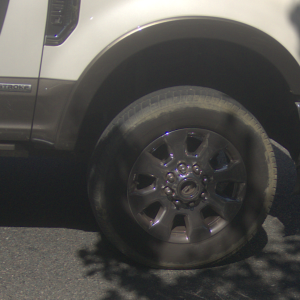
\includegraphics[width=\textwidth]{data_corrected/camera1/frame05.png}
        % \captionof{figure}{Rolling Shutter Image \(R_0\) where the corresponding Global Shutter image is at time \(t_0\)}

    \end{minipage}
    \begin{minipage}{0.06\textwidth}
        \centering
        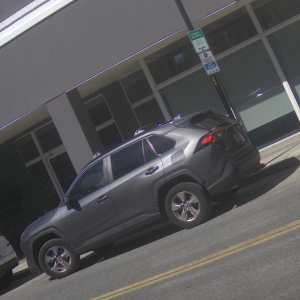
\includegraphics[width=\textwidth]{data_corrected/camera1/frame908.png}
        % \captionof{figure}{Rolling Shutter Image \(R_{N/2}\) where the corresponding Global Shutter image is at time \(t_{N/2}\)}
    \end{minipage}
    \begin{minipage}{0.06\textwidth}
        \centering
        
\includegraphics[width=\textwidth]{data_corrected/camera1/frame129.png}
        % \captionof{figure}{Rolling Shutter Image \(R_{N/2}\) where the corresponding Global Shutter image is at time \(t_{N/2}\)}
    \end{minipage}
    \begin{minipage}{0.06\textwidth}
        \centering
        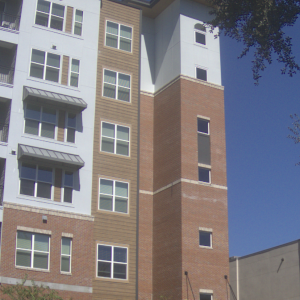
\includegraphics[width=\textwidth]{data_corrected/camera1/frame146.png}
        % \captionof{figure}{Rolling Shutter Image \(R_{N/2}\) where the corresponding Global Shutter image is at time \(t_{N/2}\)}
    \end{minipage}
    \begin{minipage}{0.06\textwidth}
        \centering
        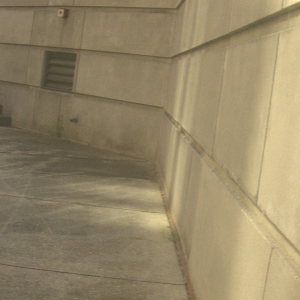
\includegraphics[width=\textwidth]{data_corrected/camera1/frame209.png}
        % \captionof{figure}{Rolling Shutter Image \(R_{N/2}\) where the corresponding Global Shutter image is at time \(t_{N/2}\)}
    \end{minipage}
    \begin{minipage}{0.06\textwidth}
        \centering
        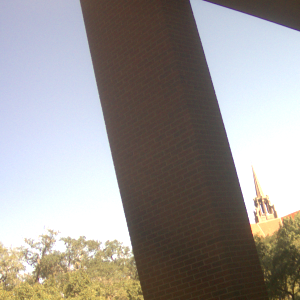
\includegraphics[width=\textwidth]{data_corrected/camera1/frame273.png}
        % \captionof{figure}{Rolling Shutter Image \(R_{N/2}\) where the corresponding Global Shutter image is at time \(t_{N/2}\)}
    \end{minipage}
    \begin{minipage}{0.06\textwidth}
        \centering
        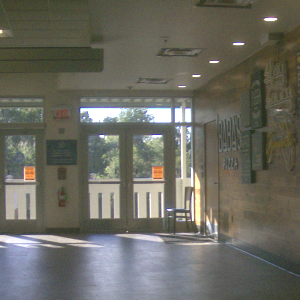
\includegraphics[width=\textwidth]{data_corrected/camera1/frame992.png}
        % \captionof{figure}{Rolling Shutter Image \(R_{N/2}\) where the corresponding Global Shutter image is at time \(t_{N/2}\)}
    \end{minipage}


    %Third Row
    \begin{minipage}{0.025\textwidth} % Narrow column for row label
        \raggedleft
        \rotatebox{90}{\text{RS}} % Vertical label for the first row
    \end{minipage}
       \begin{minipage}{0.06\textwidth}
        \centering
        
\includegraphics[width=\textwidth]{data_corrected/cam1_corrected/frame902.png}
        % \captionof{figure}{Rolling Shutter Image \(R_0\) where the corresponding Global Shutter image is at time \(t_0\)}

    \end{minipage}
    \begin{minipage}{0.06\textwidth}
        \centering
        
\includegraphics[width=\textwidth]{data_corrected/cam1_corrected/frame134.png}
        % \captionof{figure}{Rolling Shutter Image \(R_{N/2}\) where the corresponding Global Shutter image is at time \(t_{N/2}\)}
    \end{minipage}
    \begin{minipage}{0.06\textwidth}
        \centering
        
\includegraphics[width=\textwidth]{data_corrected/cam1_corrected/frame28.png}
        % \captionof{figure}{Rolling Shutter Image \(R_{N/2}\) where the corresponding Global Shutter image is at time \(t_{N/2}\)}
    \end{minipage}
    \begin{minipage}{0.06\textwidth}
        \centering
        
\includegraphics[width=\textwidth]{data_corrected/cam1_corrected/frame32.png}
        % \captionof{figure}{Rolling Shutter Image \(R_{N/2}\) where the corresponding Global Shutter image is at time \(t_{N/2}\)}
    \end{minipage}
    \begin{minipage}{0.06\textwidth}
        \centering
        
\includegraphics[width=\textwidth]{data_corrected/cam1_corrected/frame383.png}
        % \captionof{figure}{Rolling Shutter Image \(R_{N/2}\) where the corresponding Global Shutter image is at time \(t_{N/2}\)}
    \end{minipage}
    \begin{minipage}{0.06\textwidth}
        \centering
        
\includegraphics[width=\textwidth]{data_corrected/cam1_corrected/frame471.png}
        % \captionof{figure}{Rolling Shutter Image \(R_{N/2}\) where the corresponding Global Shutter image is at time \(t_{N/2}\)}
    \end{minipage}
    \begin{minipage}{0.06\textwidth}
        \centering
        
\includegraphics[width=\textwidth]{data_corrected/cam1_corrected/frame53.png}
        % \captionof{figure}{Rolling Shutter Image \(R_{N/2}\) where the corresponding Global Shutter image is at time \(t_{N/2}\)}
    \end{minipage}


    %fourth row
    \begin{minipage}{0.025\textwidth} % Narrow column for row label
        \raggedleft
        \rotatebox{90}{\text{GS}} % Vertical label for the first row
    \end{minipage}
   \begin{minipage}{0.06\textwidth}
        \centering
        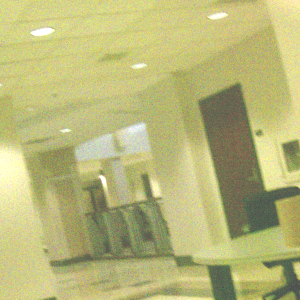
\includegraphics[width=\textwidth]{data_corrected/camera1/frame902.png}
        % \captionof{figure}{Rolling Shutter Image \(R_0\) where the corresponding Global Shutter image is at time \(t_0\)}

    \end{minipage}
    \begin{minipage}{0.06\textwidth}
        \centering
        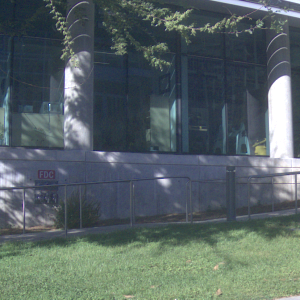
\includegraphics[width=\textwidth]{data_corrected/camera1/frame134.png}
        % \captionof{figure}{Rolling Shutter Image \(R_{N/2}\) where the corresponding Global Shutter image is at time \(t_{N/2}\)}
    \end{minipage}
    \begin{minipage}{0.06\textwidth}
        \centering
        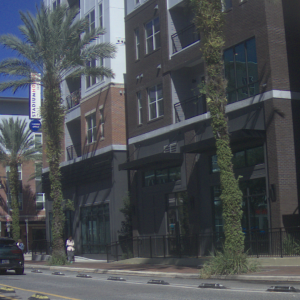
\includegraphics[width=\textwidth]{data_corrected/camera1/frame28.png}
        % \captionof{figure}{Rolling Shutter Image \(R_{N/2}\) where the corresponding Global Shutter image is at time \(t_{N/2}\)}
    \end{minipage}
    \begin{minipage}{0.06\textwidth}
        \centering
        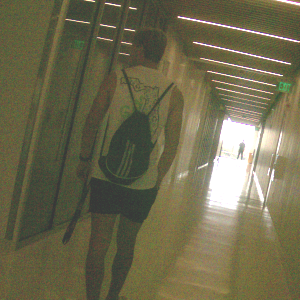
\includegraphics[width=\textwidth]{data_corrected/camera1/frame32.png}
        % \captionof{figure}{Rolling Shutter Image \(R_{N/2}\) where the corresponding Global Shutter image is at time \(t_{N/2}\)}
    \end{minipage}
    \begin{minipage}{0.06\textwidth}
        \centering
        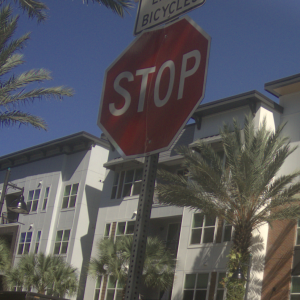
\includegraphics[width=\textwidth]{data_corrected/camera1/frame383.png}
        % \captionof{figure}{Rolling Shutter Image \(R_{N/2}\) where the corresponding Global Shutter image is at time \(t_{N/2}\)}
    \end{minipage}
    \begin{minipage}{0.06\textwidth}
        \centering
        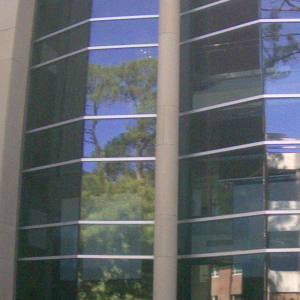
\includegraphics[width=\textwidth]{data_corrected/camera1/frame471.png}
        % \captionof{figure}{Rolling Shutter Image \(R_{N/2}\) where the corresponding Global Shutter image is at time \(t_{N/2}\)}
    \end{minipage}
    \begin{minipage}{0.06\textwidth}
        \centering
        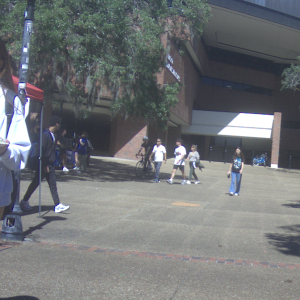
\includegraphics[width=\textwidth]{data_corrected/camera1/frame53.png}
        % \captionof{figure}{Rolling Shutter Image \(R_{N/2}\) where the corresponding Global Shutter image is at time \(t_{N/2}\)}
    \end{minipage}

    
    \caption{Highlights of the Real Dataset. Each pair of rows shows the rolling shutter capture and the corresponding global shutter capture. The dataset will be released to the public.}
    \label{fig:Real_Dataset}
    \vspace{-3mm}
\end{figure}

\subsection{Dataset Creation and Analysis}

To evaluate rolling shutter correction under large distortions, we provide three datasets containing paired RS and GS images. 

% These datasets emphasize motion profiles and distortions commonly encountered in robotic systems, and provide explicit anchor-point control for systematic study.

\vspace{1mm}
\noindent \textbf{SYN1: Synthetic Benchmark.}  
\textit{SYN1} contains RS–GS pairs rendered in Blender \cite{villar2021learning}. Each single-view scene (table fan, ceiling fan, propeller plane) includes two GS images for different anchor points and eight RS variants with increasing distortion, producing $(8 + 2)\times200 = 2000$ images per scene. 

% Randomization in lighting, colors, and textures ensures appearance diversity. To prevent overfitting, we hold out specific blade orientations (15° intervals) for testing.

\vspace{1mm}
\noindent \textbf{SYN2: Realistic RS Simulation.}  
\textit{SYN2} introduces realistic motions and textures while maintaining full control over RS effects. RS frames are synthesized from the high-speed X4K1000FPS dataset \cite{X4K} by row-wise stitching of consecutive GS frames. This method allows the selection of multiple anchor points for a single RS image.  The dataset includes \textbf{22{,}040} GS frames and \textbf{4{,}408} RS images, covering a variety of motions and scene types.

% Each RS image corresponds to five GS frames, defining five anchor points per sequence.

\noindent \textbf{REAL: Collocated RS-GS Capture.}
\textit{REAL} is a real-world dataset captured using a \textbf{dual-camera collocated system} (Fig.~\ref{fig:camera}), where rolling-shutter and global-shutter cameras are beam-splitter-aligned and hardware-synchronized. Varying trigger delays provides explicit control of the anchor point, producing multiple RS-GS pairs per scene. The dataset contains ~40k image pairs at 300×300 resolution (20k outdoor, 10k indoor, 10k additional for anchor point ablation). Optical-flow analysis (Fig.~\ref{fig:flow_bar}) shows that \textbf{REAL} exhibits the largest motion among RS datasets, making it suitable for evaluating large-distortion RS correction and depth estimation. 

% The system is attachable to a Puppy-Pi robot for legged-robot experiments
\begin{figure}[t!]
    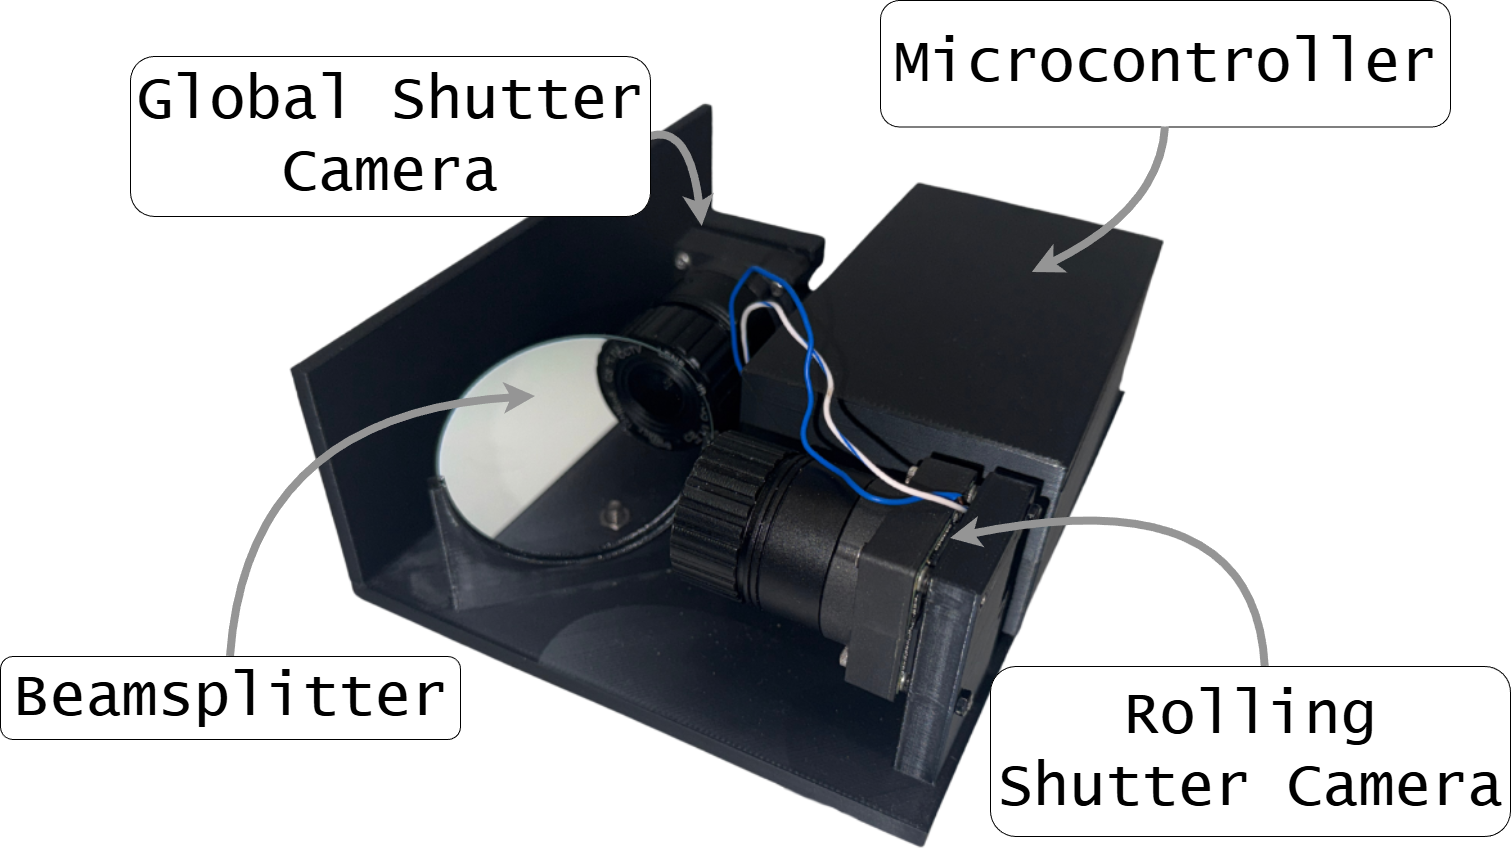
\includegraphics[width=0.55\columnwidth]{Figures/camera_diagram.drawio.png}
    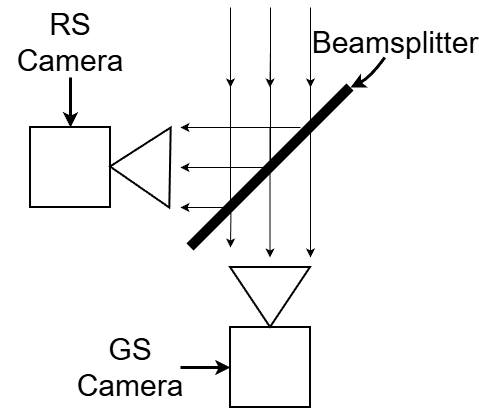
\includegraphics[width=0.4\columnwidth]{Figures/ray_diagram.drawio.png}
    \caption{Collocated RS–GS camera setup used for REAL. Hardware synchronization allows explicit control of anchor points for each capture. This device will be provided as a demo if accepted.}
    \label{fig:camera}
    \vspace{-2mm}
\end{figure}



\begin{figure*}[!bh]
    \centering

    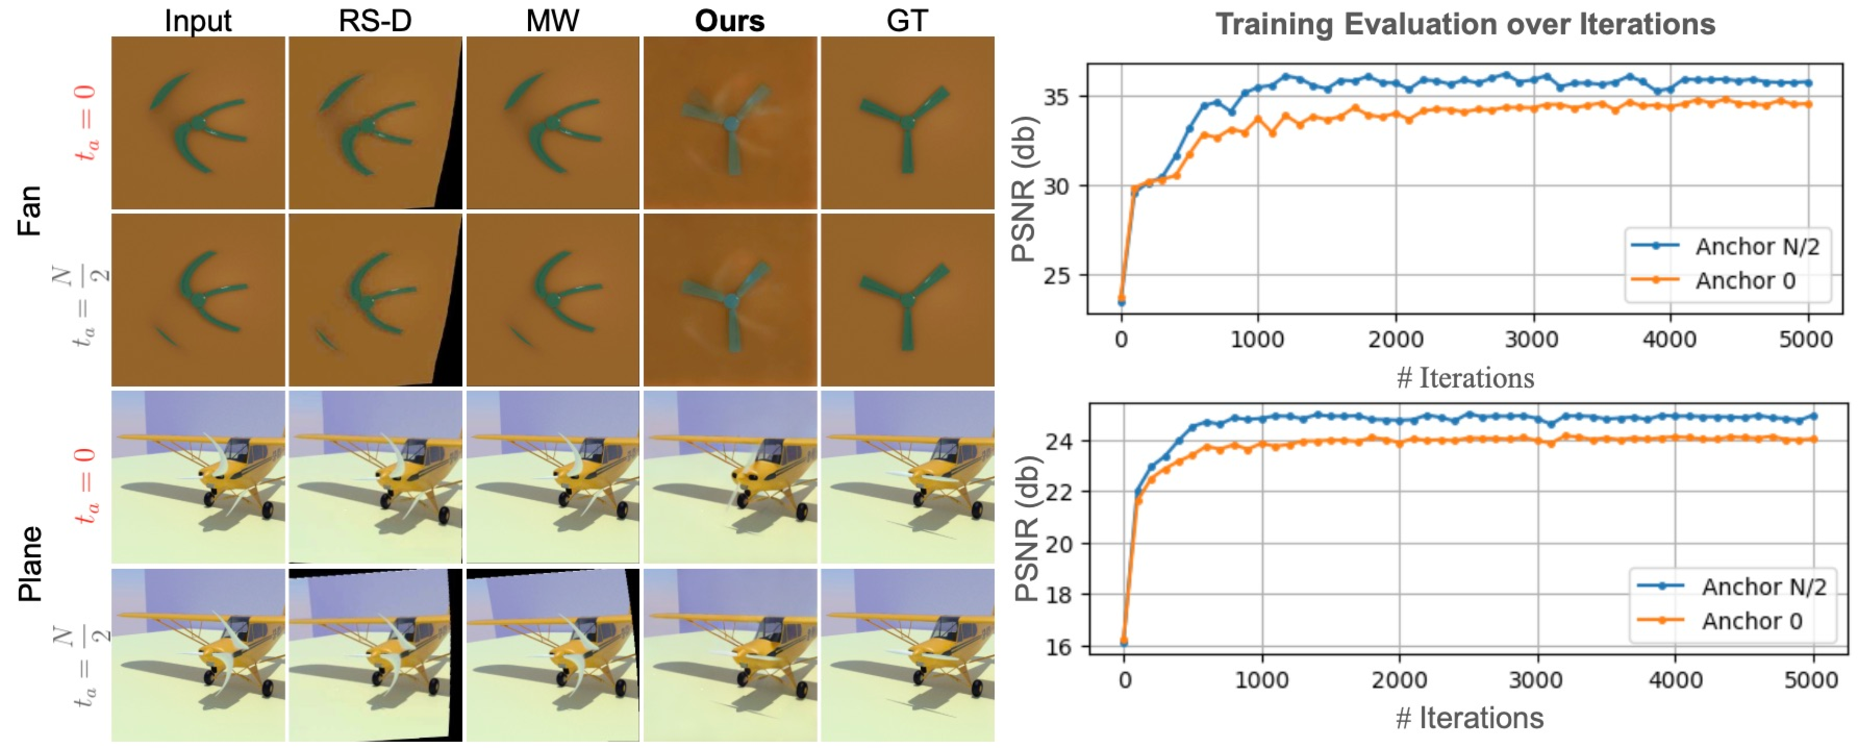
\includegraphics[width=\textwidth]{Results/SYNTH1.pdf}
    \caption{
    Results on SYN1 comparing RS-Diffusion \cite{RS-Diffusion}, Manhattan World \cite{Manhattan}, and our method under two anchor-point choices ($t_a=0$, $t_a=\frac{N}{2}$). PSNR curves show validation performance per anchor-point.
    % Visualization off our of the models run on synthetic data (\textbf{SYN1}). Each column corresponds to a method, and each row to a scene (Fan, Plane). Each scene shows the input with two anchors ($t_a=0$ and $t_a=\frac{N}{2}$), compared against RS-Diffusion \cite{RS-Diffusion}, Manhattan World \cite{Manhattan}, our model outputs, and ground truth. The PSNR curves on the right show training performance over iterations for each scene. %\JI{This figure needs a lot of revision}
    }
    \label{fig:rotated_fig_sidepsnr}
    \vspace{-4mm}
\end{figure*}
    % \begin{minipage}{0.6\textwidth} % LEFT: Images
    %     %---------------- Header Row ----------------%
    %     \hspace{.09\textwidth}
    %     \begin{minipage}{0.16\textwidth}\centering\textbf{Input}\end{minipage}
    %     \begin{minipage}{0.16\textwidth}\centering\textbf{RS-D} \cite{RS-Diffusion}\end{minipage}
    %     \begin{minipage}{0.16\textwidth}\centering\textbf{MW} \cite{Manhattan}\end{minipage}
    %     \begin{minipage}{0.16\textwidth}\centering\textbf{Ours}\end{minipage}
    %     \begin{minipage}{0.16\textwidth}\centering\textbf{GT}\end{minipage}

    %     \vspace{2mm}

    %     %---------------- FAN EXTREME ----------------%
    %     \begin{minipage}{0.02\textwidth}\rotatebox{90}{\textbf{Fan}}\end{minipage}
    %     \hspace{0.01\textwidth}
    %     \begin{minipage}{0.04\textwidth}
    %         \centering
    %         % \vspace{5mm}
    %         \rotatebox{90}{\textcolor{red}{$t_a = 0$}}\\[3mm]
    %         % \vspace{10mm}
    %         \rotatebox{90}{\textcolor{green}{$t_a = \frac{N}{2}$}}
    %     \end{minipage}
    %     \begin{minipage}{0.16\textwidth}\centering
    %         
\includegraphics[width=\textwidth]{Results/extreme/fan_extreme/start/0000.png}\\
    %         
\includegraphics[width=\textwidth]{Results/extreme/fan_extreme/center/0000.png}
    %     \end{minipage}
    %     \begin{minipage}{0.16\textwidth}\centering
    %         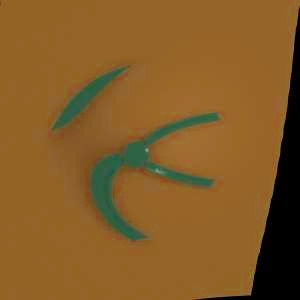
\includegraphics[width=\textwidth]{Results/RS-Diffusion/fs.jpg}\\
    %         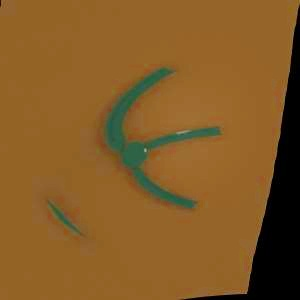
\includegraphics[width=\textwidth]{Results/RS-Diffusion/fc.jpg}
    %     \end{minipage}
    %     \begin{minipage}{0.16\textwidth}\centering
    %         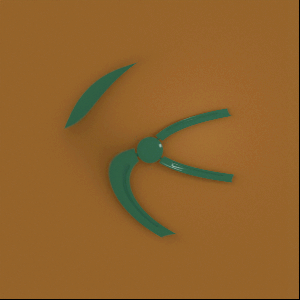
\includegraphics[width=\textwidth]{Results/manhattan/fs.png}\\
    %         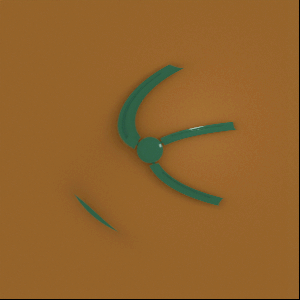
\includegraphics[width=\textwidth]{Results/manhattan/fc.png}
    %     \end{minipage}
    %     \begin{minipage}{0.16\textwidth}\centering
    %         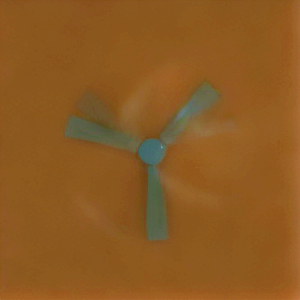
\includegraphics[width=\textwidth]{Results/extreme/fan_extreme/start/fan_extreme_test_RS0.8_START_0000.png}\\
    %         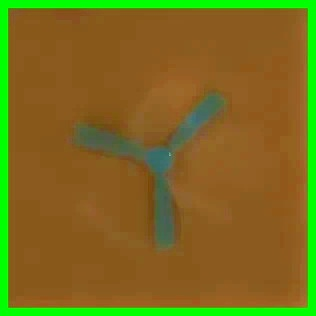
\includegraphics[width=\textwidth]{Results/extreme/fan_extreme/center/0000_green.jpg}
    %     \end{minipage}
    %     \begin{minipage}{0.16\textwidth}\centering
    %         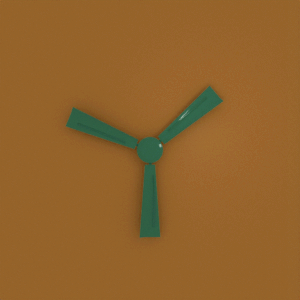
\includegraphics[width=\textwidth]{Results/extreme/fan_extreme/0000.png}\\
    %         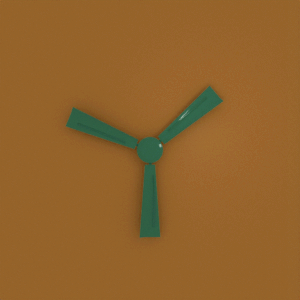
\includegraphics[width=\textwidth]{Results/extreme/fan_extreme/0000.png}
    %     \end{minipage}
    %     \vspace{0mm}
        
    %     %---------------- PLANE EXTREME ----------------%
    %     \begin{minipage}{0.02\textwidth}\rotatebox{90}{\textbf{Plane}}\end{minipage}
    %     \hspace{0.01\textwidth}
    %     \begin{minipage}{0.04\textwidth}
    %         \centering
    %         \vspace{5mm}
    %         \rotatebox{90}{\textcolor{red}{$t_a = 0$}}\\[3mm]
    %         % \vspace{13mm}
    %         \rotatebox{90}{\textcolor{green}{$t_a = \frac{N}{2}$}}
    %     \end{minipage}
    %     \begin{minipage}{0.16\textwidth}\centering
    %         
\includegraphics[width=\textwidth]{Results/extreme/plane_extreme/start/0000.png}\\
    %         
\includegraphics[width=\textwidth]{Results/extreme/plane_extreme/center/0000.png}
    %     \end{minipage}
    %     \begin{minipage}{0.16\textwidth}\centering
    %         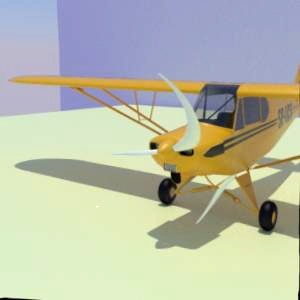
\includegraphics[width=\textwidth]{Results/RS-Diffusion/ps.jpg}\\
    %         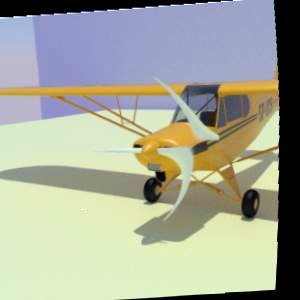
\includegraphics[width=\textwidth]{Results/RS-Diffusion/pc.jpg}
    %     \end{minipage}
    %     \begin{minipage}{0.16\textwidth}\centering
    %         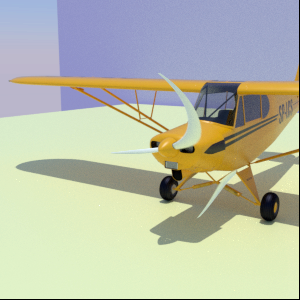
\includegraphics[width=\textwidth]{Results/manhattan/ps.png}\\
    %         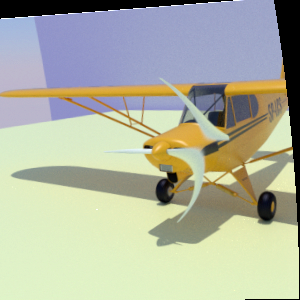
\includegraphics[width=\textwidth]{Results/manhattan/pc.png}
    %     \end{minipage}
    %     \begin{minipage}{0.16\textwidth}\centering
    %         
\includegraphics[width=\textwidth]{Results/extreme/plane_extreme/start/0000_pred.png}\\
    %         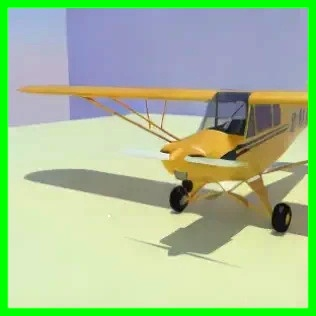
\includegraphics[width=\textwidth]{Results/extreme/plane_extreme/center/0000_pred_green.jpg}
    %     \end{minipage}
    %     \begin{minipage}{0.16\textwidth}\centering
    %         
\includegraphics[width=\textwidth]{Results/extreme/plane_extreme/0000.png}\\
    %         
\includegraphics[width=\textwidth]{Results/extreme/plane_extreme/0000.png}
    %     \end{minipage}
    % \end{minipage}%
    % % \hfill
    % \begin{minipage}{0.4\textwidth} % RIGHT: PSNR plots
    %     \centering
    %     \vspace{5mm}
    %     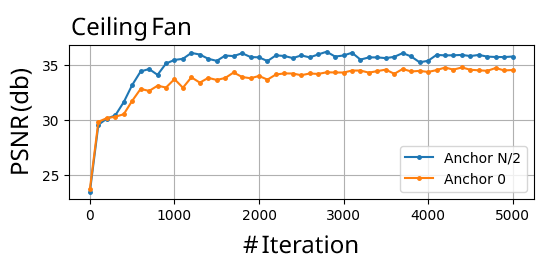
\includegraphics[width=\textwidth]{Results/fan/fan_psnr.png}\\
    %     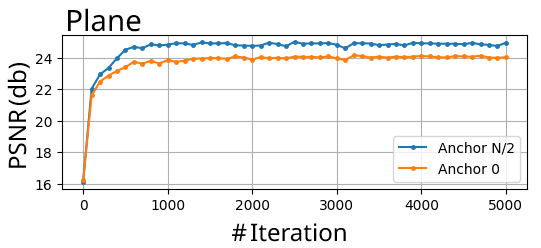
\includegraphics[width=\textwidth]{Results/Plane/plane_psnr.png}
    % \end{minipage}




\begin{figure}[t!]
    \centering
    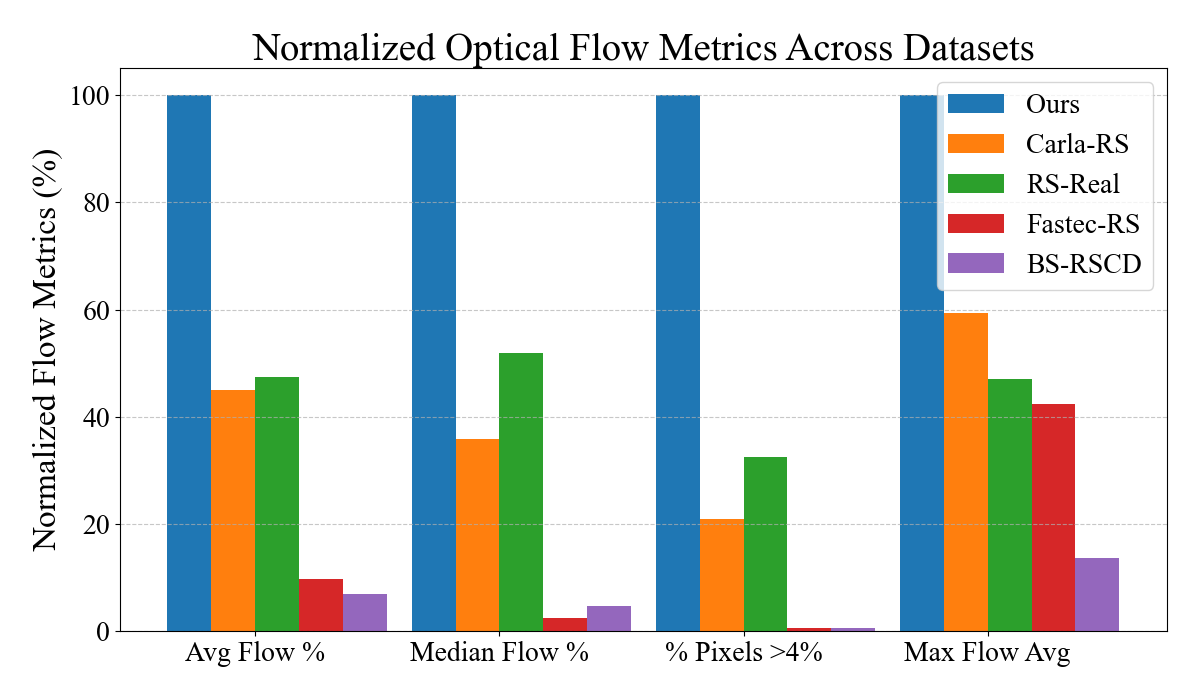
\includegraphics[width=\columnwidth]{collage/Figure_1.png}%
    \vspace{-2mm}
    \caption{Optical-flow motion statistics for RS datasets. For our dataset, the percentage of pixels with greater than 2\%, 6\%, and 10\% flow was more than double that of the other datasets. \textbf{No other dataset matches our egocentric motion, allowing us to model legged robots and other mobile systems.}}
    \label{fig:flow_bar}
    \vspace{-2mm}
\end{figure}





\subsection{Integration of Vision Foundation Models}

To address RS correction and monocular depth estimation, we leverage pre-existing vision foundation models (VFMs). Our pipeline consists of two sequential stages:




\begin{enumerate}
    \item \textbf{RS Correction Stage:} We adopt a Marigold U-Net~\cite{StableDiffusion} trained to map RS images to corresponding GS frames. The model operates on RGB images and focuses on removing row-wise distortions while preserving structure.
    
    \item \textbf{Monocular Depth Estimation Stage:} Corrected RS frames from the first stage are passed to a transformer-based Depth-Anything-V2~\cite{DepthAnything}. This stage produces dense depth maps, benefiting from the reduction in RS-induced geometric distortions. 
\end{enumerate}
\draft{Since metric depth ground truth is unavailable for the RS-GS datasets, we evaluate depth consistency relative to a frozen Depth-Anything-V2 teacher operating on the GS image. This measures preservation of geometric structure after RS correction rather than absolute metric depth accuracy. The teacher provides a consistent reference across all methods, isolating errors introduced by rolling shutter distortions.
}

\noindent \textbf{Pipeline Details.}  
The stages are trained sequentially: first, the Marigold U-Net is trained for RS correction; second, the corrected outputs are used to  fine-tune the depth model. 

% We experimented with different VFM configurations and found that sequentially applying two distinct VFMs yields better depth accuracy than either model alone. 

\vspace{1mm}
\noindent \textbf{Training Setup.}  
Both stages are trained using our RS-GS paired datasets (\textbf{SYN1}, \textbf{SYN2}, \textbf{REAL}). Standard image augmentation is applied, and losses include MSE loss for RS correction and scale invariant loss for Depth-Anything-V2. 

% All other architectural components (e.g., U-Net layers, transformer blocks) remain unchanged from the original VFMs, highlighting that improvements derive from task-specific training and anchor-point alignment.

% \vspace{1mm}
% \noindent \textbf{Purpose of VFM Integration.}  
% We use Vision Foundation Models (VFMs) to leverage strong priors for RGB reconstruction and monocular depth estimation, allowing us to isolate and analyze rolling shutter distortions and anchor-point effects. Depth-Anything is employed as a second-stage evaluator to assess structural and geometric consistency of the corrected outputs, rather than focusing on high-frequency photometric artifacts. This enables evaluation of rolling shutter behavior at a geometric level relevant to depth estimation.

\draft{\subsection{Comparisons and Baselines}
All trainable baselines were fine-tuned on the training splits used by our method whenever training code and model weights were publicly available \cite{RS-Diffusion}. For methods whose temporal reference is fixed by design, results are reported using the authors' original formulation. Evaluation was performed on identical testing data. Baselines of the author's original implementations are included alongside fine-tuned implementations.
}
% \begin{figure*}[t!]
%     \vspace{2mm}  % vertical space + line break
%     \centering
% \parbox{0.04\textwidth}{\centering {}}
% \parbox{0.095\textwidth}{\centering \textbf{SYN2}}
% \rule{0.6pt}{.3cm}
% \parbox{0.725\textwidth}{\centering \textbf{REAL / RS-GS}}


    
%     % Input Image
%     \begin{minipage}{0.05\textwidth} % Narrow column for row label
%         \raggedleft
%         \rotatebox{90}{\text{Input Image}} % Vertical label for the first row
%     \end{minipage}
%     \begin{minipage}{0.115\textwidth}
%         \vspace{0.05cm}
%         \centering
%         
\includegraphics[width=\textwidth]{X4K_data/input/occ068.802_f3921.png}
%     \end{minipage}
%     \begin{minipage}{0.115\textwidth}
%         \vspace{0.05cm}
%         \centering
%         
\includegraphics[width=\textwidth]{Collocated_Collage/input/frame08.png}
%     \end{minipage}
%     \begin{minipage}{0.115\textwidth}
%         \vspace{0.05cm}
%         \centering
%         
\includegraphics[width=\textwidth]{Collocated_Collage/10-20-vis/input/frame184.png}
%     \end{minipage}
%     \begin{minipage}{0.115\textwidth}
%         \vspace{0.05cm}
%         \centering
%         
\includegraphics[width=\textwidth]{Collocated_Collage/input/frame958.png}
%     \end{minipage}
%     \begin{minipage}{0.115\textwidth}
%         \vspace{0.05cm}
%         \centering
%         
\includegraphics[width=\textwidth]{Collocated_Collage/10-20-vis/input/frame264.png}
%     \end{minipage}
%     \begin{minipage}{0.115\textwidth}
%         \vspace{0.05cm}
%         \centering
%         
\includegraphics[width=\textwidth]{Collocated_Collage/input/frame96.png}
%     \end{minipage}
%     \begin{minipage}{0.115\textwidth}
%         \vspace{0.05cm}
%         \centering
%         
\includegraphics[width=\textwidth]{Collocated_Collage/10-20-vis/input/frame691.png}
%     \end{minipage}
%     \hspace{0.05\textwidth}

%     % Manhattan
%     \begin{minipage}{0.05\textwidth} % Narrow column for row label
%         \raggedleft
%         \rotatebox{90}{\text{MW \cite{Manhattan}}} % Vertical label for the first row
%     \end{minipage}
%     \begin{minipage}{0.115\textwidth}
%         \vspace{0.05cm}
%         \centering
%         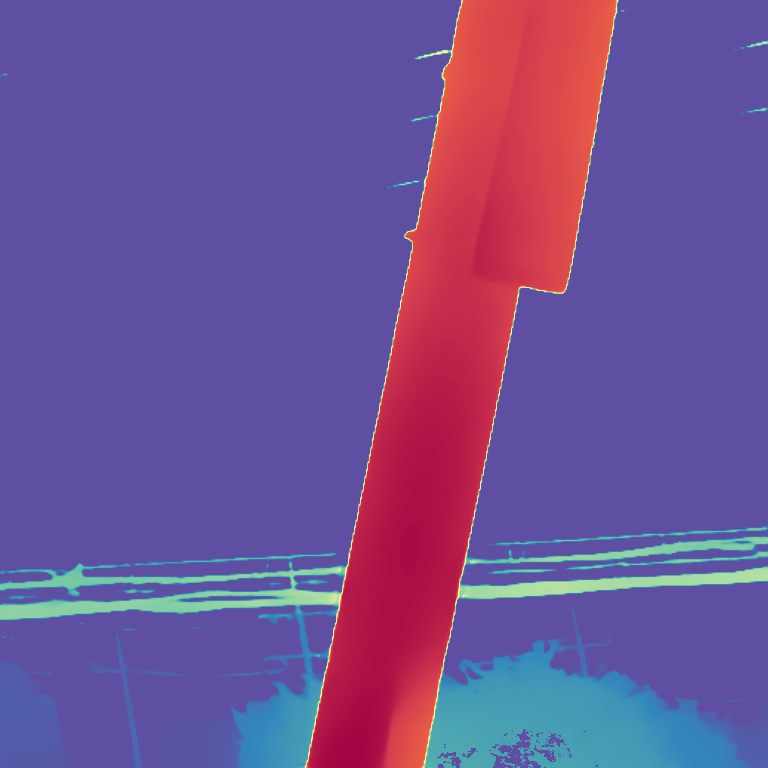
\includegraphics[width=\textwidth]{Collocated_Collage/mw_depth/manhattan_world/068mw.png}
%     \end{minipage}
%     \begin{minipage}{0.115\textwidth}
%         \vspace{0.05cm}
%         \centering
%         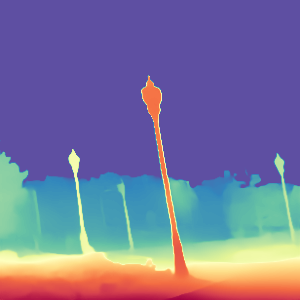
\includegraphics[width=\textwidth]{Collocated_Collage/mw_depth/output_frame08.png}
%     \end{minipage}
%     \begin{minipage}{0.115\textwidth}
%         \vspace{0.05cm}
%         \centering
%         
\includegraphics[width=\textwidth]{Collocated_Collage/mw_depth/manhattan_world/frame184mw.png}
%     \end{minipage}
%     \begin{minipage}{0.115\textwidth}
%         \vspace{0.05cm}
%         \centering
%         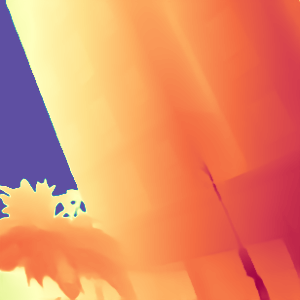
\includegraphics[width=\textwidth]{Collocated_Collage/mw_depth/output_frame958.png}
%     \end{minipage}
%     \begin{minipage}{0.115\textwidth}
%         \vspace{0.05cm}
%         \centering
%         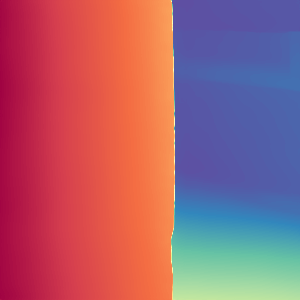
\includegraphics[width=\textwidth]{Collocated_Collage/mw_depth/manhattan_world/frame264mw.png}
%     \end{minipage}
%     \begin{minipage}{0.115\textwidth}
%         \vspace{0.05cm}
%         \centering
%         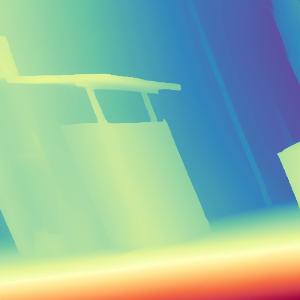
\includegraphics[width=\textwidth]{Collocated_Collage/mw_depth/manhattan_world/frame96mw.png}
%     \end{minipage}
%     \begin{minipage}{0.115\textwidth}
%         \vspace{0.05cm}
%         \centering
%         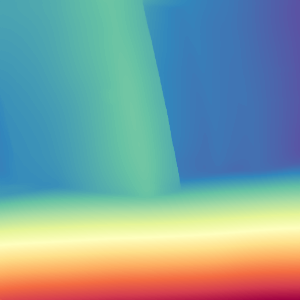
\includegraphics[width=\textwidth]{Collocated_Collage/mw_depth/manhattan_world/frame691mw.png}
%     \end{minipage}
%     \hspace{0.05\textwidth}

%     % RS-Homo
%     \begin{minipage}{0.05\textwidth} % Narrow column for row label
%         \raggedleft
%         \rotatebox{90}{\text{RS-HM \cite{RS-Homo}}} % Vertical label for the first row
%     \end{minipage}
%     \begin{minipage}{0.115\textwidth}
%         \vspace{0.05cm}
%         \centering
%         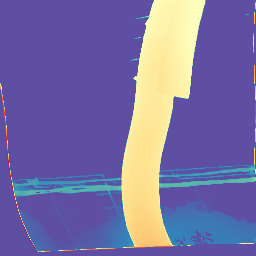
\includegraphics[width=\textwidth]{Collocated_Collage/RS-Homo_depth/RS-Homo/pred_occ068.802_f3921.png}
%     \end{minipage}
%     \begin{minipage}{0.115\textwidth}
%         \vspace{0.05cm}
%         \centering
%         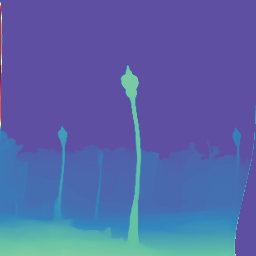
\includegraphics[width=\textwidth]{Collocated_Collage/RS-Homo_depth/RS-Homo/pred_frame08.png}
%     \end{minipage}
%     \begin{minipage}{0.115\textwidth}
%         \vspace{0.05cm}
%         \centering
%         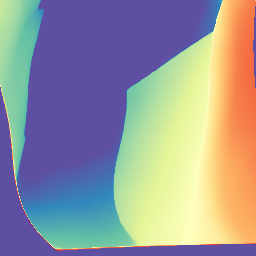
\includegraphics[width=\textwidth]{Collocated_Collage/RS-Homo_depth/RS-Homo/pred_frame184.png}
%     \end{minipage}
%     \begin{minipage}{0.115\textwidth}
%         \vspace{0.05cm}
%         \centering
%         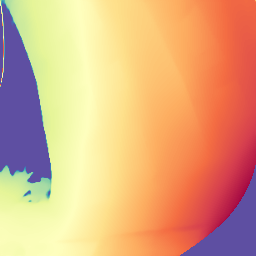
\includegraphics[width=\textwidth]{Collocated_Collage/RS-Homo_depth/RS-Homo/pred_frame958.png}
%     \end{minipage}
%     \begin{minipage}{0.115\textwidth}
%         \vspace{0.05cm}
%         \centering
%         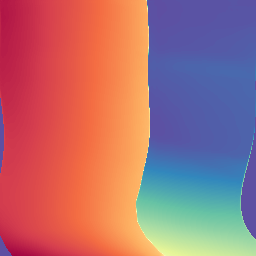
\includegraphics[width=\textwidth]{Collocated_Collage/RS-Homo_depth/RS-Homo/pred_frame264.png}
%     \end{minipage}
%     \begin{minipage}{0.115\textwidth}
%         \vspace{0.05cm}
%         \centering
%         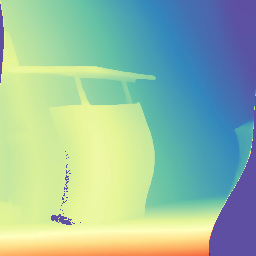
\includegraphics[width=\textwidth]{Collocated_Collage/RS-Homo_depth/RS-Homo/pred_frame96.png}
%     \end{minipage}
%     \begin{minipage}{0.115\textwidth}
%         \vspace{0.05cm}
%         \centering
%         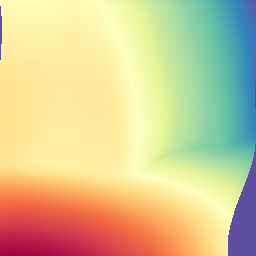
\includegraphics[width=\textwidth]{Collocated_Collage/RS-Homo_depth/RS-Homo/pred_frame691.png}
%     \end{minipage}
%     \hspace{0.05\textwidth}

%     % RS-Diffusion
%     \begin{minipage}{0.05\textwidth} % Narrow column for row label
%         \raggedleft
%         \rotatebox{90}{\text{RS-D FT \cite{RS-Diffusion}}} % Vertical label for the first row
%     \end{minipage}
%     \begin{minipage}{0.115\textwidth}
%         \vspace{0.05cm}
%         \centering
%         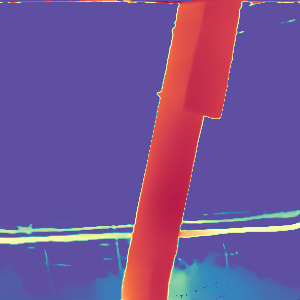
\includegraphics[width=\textwidth]{Collocated_Collage/10-20-vis/rs-diff/occ068.802_f3921 (2).png}
%     \end{minipage}
%     \begin{minipage}{0.115\textwidth}
%         \vspace{0.05cm}
%         \centering
%         
\includegraphics[width=\textwidth]{Collocated_Collage/10-20-vis/rs-diff/frame08.png}
%     \end{minipage}
%     \begin{minipage}{0.115\textwidth}
%         \vspace{0.05cm}
%         \centering
%         
\includegraphics[width=\textwidth]{Collocated_Collage/10-20-vis/rs-diff/frame184.png}
%     \end{minipage}
%     \begin{minipage}{0.115\textwidth}
%         \vspace{0.05cm}
%         \centering
%         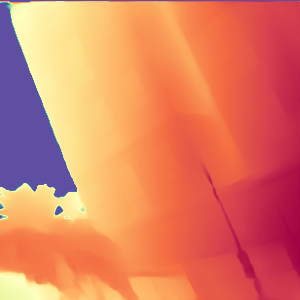
\includegraphics[width=\textwidth]{Collocated_Collage/10-20-vis/rs-diff/frame958.png}
%     \end{minipage}
%     \begin{minipage}{0.115\textwidth}
%         \vspace{0.05cm}
%         \centering
%         
\includegraphics[width=\textwidth]{Collocated_Collage/10-20-vis/rs-diff/frame264.png}
%     \end{minipage}
%     \begin{minipage}{0.115\textwidth}
%         \vspace{0.05cm}
%         \centering
%         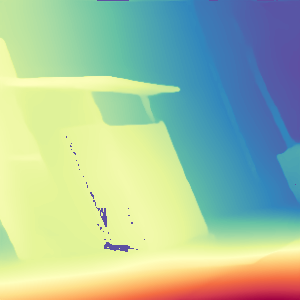
\includegraphics[width=\textwidth]{Collocated_Collage/10-20-vis/rs-diff/frame96.png}
%     \end{minipage}
%     \begin{minipage}{0.115\textwidth}
%         \vspace{0.05cm}
%         \centering
%         
\includegraphics[width=\textwidth]{Collocated_Collage/10-20-vis/rs-diff/frame691.png}
%     \end{minipage}
%     \hspace{0.05\textwidth}

%     % Ours
%     \begin{minipage}{0.05\textwidth} % Narrow column for row label
%         \raggedleft
%         \rotatebox{90}{\text{Ours}} % Vertical label for the first row
%     \end{minipage}
%     \begin{minipage}{0.115\textwidth}
%         \vspace{0.05cm}
%         \centering
%         
\includegraphics[width=\textwidth]{X4K_data/fine_tuned_depth/occ068.802_f3921_pred.png}
%     \end{minipage}
%     \begin{minipage}{0.115\textwidth}
%         % \vspace{0.05cm}
%         \centering
%         
\includegraphics[width=\textwidth]{Collocated_Collage/output_bw_color/frame08.png}
%     \end{minipage}
%     \begin{minipage}{0.115\textwidth}
%         \vspace{0.05cm}
%         \centering
%         
\includegraphics[width=\textwidth]{Collocated_Collage/10-20-vis/output/frame184.png}
%     \end{minipage}
%     \begin{minipage}{0.115\textwidth}
%         \vspace{0.05cm}
%         \centering
%         
\includegraphics[width=\textwidth]{Collocated_Collage/output_bw_color/frame958.png}
%     \end{minipage}
%     \begin{minipage}{0.115\textwidth}
%         \vspace{0.05cm}
%         \centering
%         
\includegraphics[width=\textwidth]{Collocated_Collage/10-20-vis/output/frame264.png}
%     \end{minipage}
%     \begin{minipage}{0.115\textwidth}
%         \vspace{0.05cm}
%         \centering
%         
\includegraphics[width=\textwidth]{Collocated_Collage/output_bw_color/frame96.png}
%     \end{minipage}
%     \begin{minipage}{0.115\textwidth}
%         \vspace{0.05cm}
%         \centering
%         
\includegraphics[width=\textwidth]{Collocated_Collage/10-20-vis/output/frame691.png}
%     \end{minipage}
%     \hspace{0.05\textwidth}

%     % Ground Truth
%     \begin{minipage}{0.05\textwidth} % Narrow column for row label
%         \raggedleft
%         \rotatebox{90}{\text{Ground Truth}} % Vertical label for the first row
%     \end{minipage}
%     \begin{minipage}{0.115\textwidth}
%         % \vspace{0.05cm}
%         \centering
%         
\includegraphics[width=\textwidth]{X4K_data/gt_depth/occ068.802_f3921.png}
%     \end{minipage}
%     \begin{minipage}{0.115\textwidth}
%         \vspace{0.05cm}
%         \centering
%         
\includegraphics[width=\textwidth]{Collocated_Collage/gt_depth_color/frame08.png}
%     \end{minipage}
%     \begin{minipage}{0.115\textwidth}
%         \vspace{0.05cm}
%         \centering
%         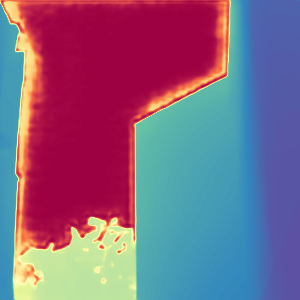
\includegraphics[width=\textwidth]{Collocated_Collage/10-20-vis/gt/frame184.png}
%     \end{minipage}
%     \begin{minipage}{0.115\textwidth}
%         \vspace{0.05cm}
%         \centering
%         
\includegraphics[width=\textwidth]{Collocated_Collage/gt_depth_color/frame958.png}
%     \end{minipage}
%     \begin{minipage}{0.115\textwidth}
%         \vspace{0.05cm}
%         \centering
%         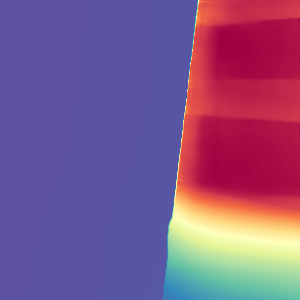
\includegraphics[width=\textwidth]{Collocated_Collage/10-20-vis/gt/frame264.png}
%     \end{minipage}
%     \begin{minipage}{0.115\textwidth}
%         \vspace{0.05cm}
%         \centering
%         
\includegraphics[width=\textwidth]{Collocated_Collage/gt_depth_color/frame96.png}
%     \end{minipage}
%     \begin{minipage}{0.115\textwidth}
%         \vspace{0.05cm}
%         \centering
%         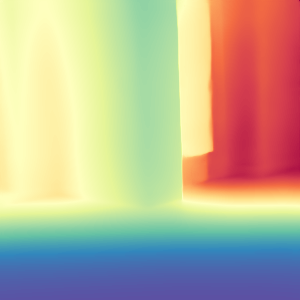
\includegraphics[width=\textwidth]{Collocated_Collage/10-20-vis/gt/frame691.png}
%     \end{minipage}
%     \hspace{0.05\textwidth}

%     \caption{Qualitative results on real scenes. From top to bottom: input image, two baseline comparison outputs, fine-tuned comparison output, our model’s output, and ground truth. Only our method produces accurate depth, demonstrating the two-stage approach preserves scene structure. \textbf{Note Column 5}, where naive affine-based rectification does not work, since the ground truth has a slanted structure. Additional visualizations and comparisons can be seen in the supplementary video.}
%     \label{fig:collocated_results}
%     \vspace{-2mm}
% \end{figure*}

\begin{figure*}
    \centering
    \vspace{0.6in}
    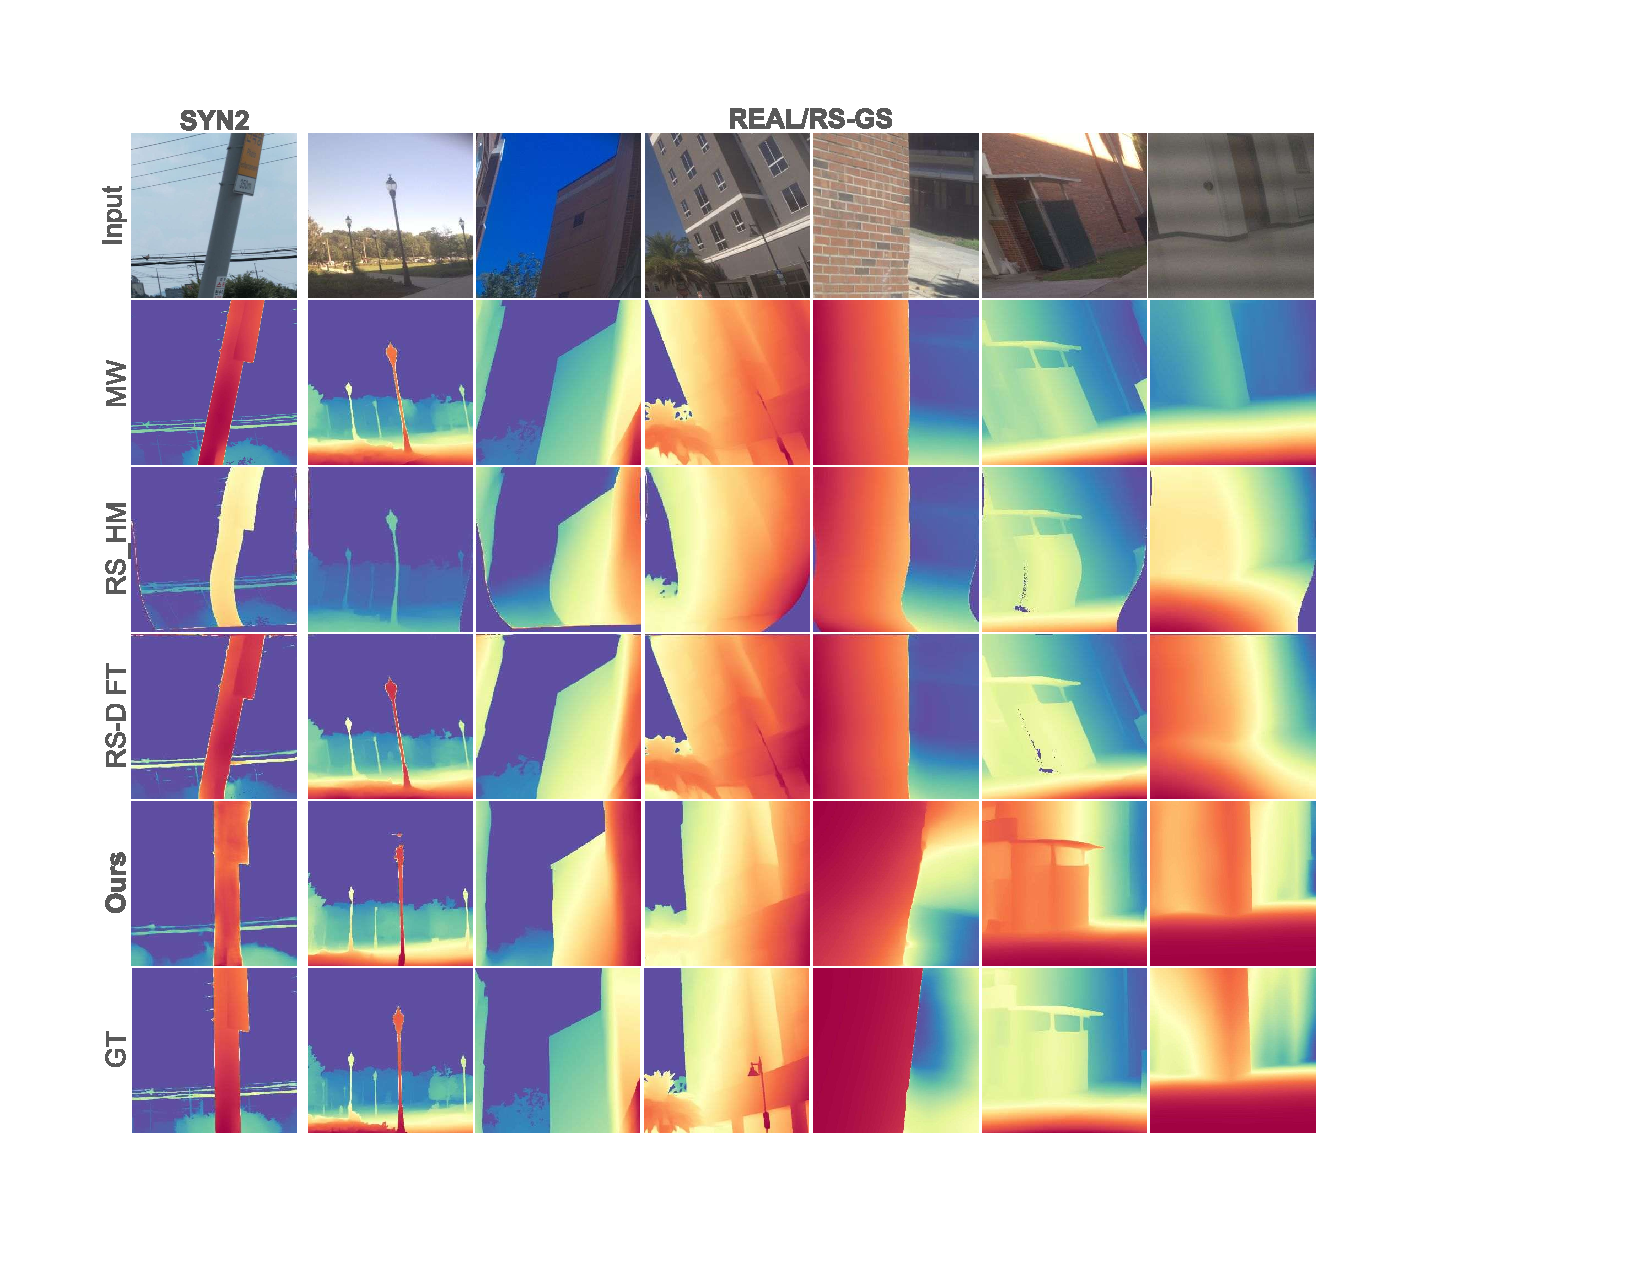
\includegraphics[width=0.8\textwidth, trim={3cm 2.5cm 7cm 3cm}]{Figures/colocated_results.pdf}%
    \vspace{1mm}
    \caption{Qualitative results on real scenes. From top to bottom: input image, two baseline comparison outputs, fine-tuned comparison output, our model’s output, and ground truth. Only our method produces accurate depth, demonstrating the two-stage approach preserves scene structure. \textbf{Note Column 5}, where naive affine-based rectification does not work since the ground truth has a slanted structure. Additional visualizations and comparisons can be seen in the supplementary video.}
    \label{fig:collocated_results}
    % \vspace{-4mm}
\end{figure*}

\section{Experimental Analyses}
\label{sec:experiments}

Our experiments were designed to validate the theoretical motivation for anchor points, evaluate VFMs on RSC, and analyze how different design choices affect rolling shutter correction and depth estimation quality. 

\subsection{Anchor Points for Controlled Synthetic Scenes}

We conduct single-scene experiments on the synthetic dataset \textbf{SYN1} to isolate the effect of anchor-point selection. Scenes exhibit rotation about the image center, suggesting an optimal anchor of $t_a=\frac{N}{2}$. Six diffusion models were trained across three scenes, comparing optimal ($t_a = \frac{N}{2}$) and suboptimal anchor points. Only models trained with the optimal anchor successfully corrected all three scenes, confirming our theoretical predictions (Fig.~\ref{fig:rotated_fig_sidepsnr}, Table \ref{table:AnchorPoint_single}). We further compare against Manhattan World~\cite{Manhattan} and RS-Diffusion~\cite{RS-Diffusion}, which struggle under extreme distortions.
% We begin with controlled single-scene experiments to isolate the effect of anchor point selection. Diffusion models were trained on individual scenes from the synthetic dataset \textbf{SYN1}, where the axis of rotation is fixed at the image center, suggesting an optimal anchor point of $t_a = \frac{N}{2}$.



% We further compared our pipeline with \textbf{Manhattan World}~\cite{Manhattan} and \textbf{RS-Diffusion}~\cite{RS-Diffusion}. These general-purpose methods struggle with the extreme distortions in SYN1, whereas our VFM pipeline preserves structure and continuity.
% \begin{table*}
%   \caption{Comparisons of different anchor points with the first stage of our two stage architecture. Three separate anchor points were tested $t_a = 0, \frac{N}{4}, \frac{N}{2}$. The models were run on the single scene datasets, the modified X4K dataset, and a subset of the real world collocated dataset. These comparisons were done on the intermediate RGB images, and $t_a = \frac{N}{2}$ outperforms all other anchor points. }
%   \centering
%   \begin{tabular}{c c c c cc c  c c  c c }
%     \hline
%        \multirow{2}{*}{Anchor} & \multicolumn{2}{c}{Ceiling Fan} & \multicolumn{2}{c}{Table Fan}& \multicolumn{2}{c}{Plane} & \multicolumn{2}{c}{X4K} & \multicolumn{2}{c}{Collocated}\\

%       &PSNR &SSIM&PSNR &SSIM&PSNR &SSIM & PSNR & SSIM & PSNR & SSIM \\
%     \hline
%       $t_a=0$& 34.93 & 0.971 & 26.82 & 0.831 & 24.21 & 0.808 &15.594 & 0.578 & 20.238 & 0.639\\
%       $t_a=\frac{N}{4}$&&&&&&&  17.291 & \textbf{0.630} & 20.292 & 0.640\\
%       $t_a=\frac{N}{2}$ & \textbf{36.21} & \textbf{0.986} & \textbf{27.57} & \textbf{0.842} & \textbf{25.02} & \textbf{0.841} & \textbf{17.733} & 0.629 & \textbf{21.778} & \textbf{0.674}\\



%     \hline
%     %3.66, 2.8, 3.35
%     %0.51, 1.32, 0.74
%   \end{tabular}

%   \label{table:AnchorPoint}
% \end{table*}

\begin{table}[th!]
  \caption{Comparisons of different anchor points with the first stage of our two-stage architecture on single-scene datasets (Ceiling Fan, Table Fan, Plane). The models were evaluated using PSNR and SSIM on intermediate RGB images. $t_a = \frac{N}{2}$ achieves the highest performance across all scenes.}
  \centering
  \setlength{\tabcolsep}{4pt} % tighten column spacing
  \begin{tabular}{c c c c c c c}
    \hline
    \multirow{2}{*}{Anchor} & \multicolumn{2}{c}{Ceiling Fan} & \multicolumn{2}{c}{Table Fan} & \multicolumn{2}{c}{Plane} \\
    & PSNR & SSIM & PSNR & SSIM & PSNR & SSIM \\
    \hline
    $t_a=0$ & 34.93 & 0.971 & 26.82 & 0.831 & 24.21 & 0.808 \\
    $t_a=\frac{N}{2}$ & \textbf{36.21} & \textbf{0.986} & \textbf{27.57} & \textbf{0.842} & \textbf{25.02} & \textbf{0.841} \\
    \hline
  \end{tabular}
  \label{table:AnchorPoint_single}
  % \vspace{-3mm}
\end{table}






% \begin{table*}[h]
%   \caption{Comparisons of PSNR, SSIM, AbsRel, and $\delta_1$ on the testing dataset used in Sect. 5.2. Our fine-tuned, two-stage architecture (U-Net, Transformer) performs better on validation than any other combination of the architectures. Values that are not possible to record (intermediate RGB metrics for one-stage architecture) are represented with NA.}
%   \centering
%   \begin{tabular}{c c  c c  c c  }
%     \hline
%       \multirow{2}{*}{Architecture} & \multirow{2}{*}{Method} &  \multicolumn{2}{c}{Intermediate RGB} & \multicolumn{2}{c}{Depth Map}\\
%      \cmidrule(lr){3-4} \cmidrule(lr){5-6} 
%       &&PSNR &SSIM  & AbsRel & $\delta_1$\\
%       \hline
%     \multirow{3}{*}{One Stage} & \cite{Marigold} & NA  & NA~ &6.047 &0.743\\
%     &\cite{DepthAnything}& NA &  NA & 0.655 & 0.243\\
%     &\cite{ecodepth}&  &   & 0.655 & 0.243\\


%     \hline
%     \multirow{3}{*}{Comparisons} & \cite{RS-Diffusion} & 20.360 & 0.559 & 0.904& 0.810\\
%     & \cite{RS-Homo} & 21.222 & 0.576 & 0.788& 0.554\\
%     & \cite{Manhattan} & 17.900 & 0.489 & 0.621& 0.377\\
    
%     \hline
%     \multirow{1}{*}{Parallel Two Stage}&\cite{Marigold}-\cite{Marigold} & 22.87  & 0.494  & 3.22 & 0.618\\
%     \hline
    
%     \multirow{2}{*}{Orthogonal Two Stage}&\cite{Marigold}-\cite{ecodepth} & 22.87 & 0.494 & 6.48 & 0.917\\
%     &Baseline \cite{Marigold}-\cite{DepthAnything} & 22.87  & 0.494 & 0.377 & 0.227\\
%     \hline
%     &\textbf{Fine Tuned (ours)}& 22.87  & 0.494 &\textbf{0.191} & \textbf{0.158}\\



%     \hline
%     %3.66, 2.8, 3.35
%     %0.51, 1.32, 0.74
%   \end{tabular}

%   \label{table:collocated_orthogonal_table}
% \end{table*}
\begin{table*}[h!]
  \caption{Comparisons of PSNR, SSIM, AbsRel, and $\delta_1$ on the testing dataset used in Sec. V-B. Our fine-tuned, two-stage architecture (U-Net, Transformer) performs better on validation than any other combination of the architectures. Values that are not possible to record (intermediate RGB metrics for one-stage architecture) are represented with NA. Comparisons of two-stage architectures with shared first stages will have repeated metrics for intermediate RGB. }
  \centering
  \setlength{\tabcolsep}{15pt} % default is usually 6pt
  \begin{tabular}{l l c c c c}
    \hline
    \multirow{2}{*}{\textbf{Architecture}} & \multirow{2}{*}{\textbf{Method}} & \multicolumn{2}{c}{Intermediate RGB} & \multicolumn{2}{c}{Depth Map}\\
    \cmidrule(lr){3-4} \cmidrule(lr){5-6}
    & & PSNR $\uparrow$& SSIM $\uparrow$& AbsRel $\downarrow$& $\delta_1 \uparrow$\\
    \hline
    \multirow{3}{*}{One Stage} & Marigold\cite{Marigold} & NA & NA & 6.047 & 0.257\\
    & Depth-Anything-V2\cite{DepthAnything} & NA & NA & 0.655 & 0.757\\
    & Eco-Depth\cite{ecodepth} & NA & NA & 0.488 & 0.676\\
    \hline
    \multirow{4}{*}{Comparisons} & RS-Diff\cite{RS-Diffusion} & 19.47 & 0.433 & 0.904 & 0.190\\
    &RS-Diff Fine-tuned\cite{RS-Diffusion} & 21.52 & 0.469 & 0.802 & 0.214\\
    & Deep RS-HM\cite{RS-Homo} & 20.75 & 0.456 & 0.788 & 0.446\\
    & Manhattan\cite{Manhattan} & 21.41 & 0.454 & 0.621 & 0.623\\
    \hline
    \multirow{1}{*}{Parallel Two Stage} & \cite{Marigold}-\cite{Marigold} & 22.87 & 0.494 & 3.22 & 0.382\\
    \hline
    \multirow{2}{*}{Orthogonal Two Stage} & \cite{Marigold}-\cite{ecodepth} & 22.87 & 0.494 & 0.506 & 0.649\\
    & Baseline \cite{Marigold}-\cite{DepthAnything} & 22.87 & 0.494 & 0.377 & 0.773\\
    \hline
    & \textbf{Fine Tuned (ours)} & \textbf{22.87} & \textbf{0.494} & \textbf{0.191} & \textbf{0.842}\\
    \hline
  \end{tabular}
  \label{table:collocated_orthogonal_table}
  \vspace{-2mm}
\end{table*}



\subsection{Anchor Points in General Realistic Scenes}
Next, we evaluated the full two-stage pipeline, RS correction followed by monocular depth estimation. 

\vspace{1mm}
\noindent \textbf{Synthetic Results.}  
On the X4K-based dataset~\cite{X4K}, we trained models using different anchor-point choices spanning the exposure window. Performance consistently peaked near the temporal midpoint, with $t_a=\frac{N}{2}$ yielding the highest PSNR across training (Fig.~\ref{fig:PSNR_X4K}). Visual comparisons show cleaner reconstructions and more consistent depth than prior RS correction methods (Fig.~\ref{fig:collocated_results}).



\vspace{1mm}
\noindent \textbf{Real-World Results.}  
On the novel \textbf{REAL} dataset, our pipeline consistently outperformed baseline RS correction models and Depth-Anything-V2 in both RGB fidelity and depth accuracy (Table~\ref{table:collocated_orthogonal_table}). PSNR improvements are most pronounced in high-motion sequences, demonstrating robustness to large RS distortions (Fig.~\ref{fig:flow_vs_perf}). 

\begin{figure}[b!]
    \centering
    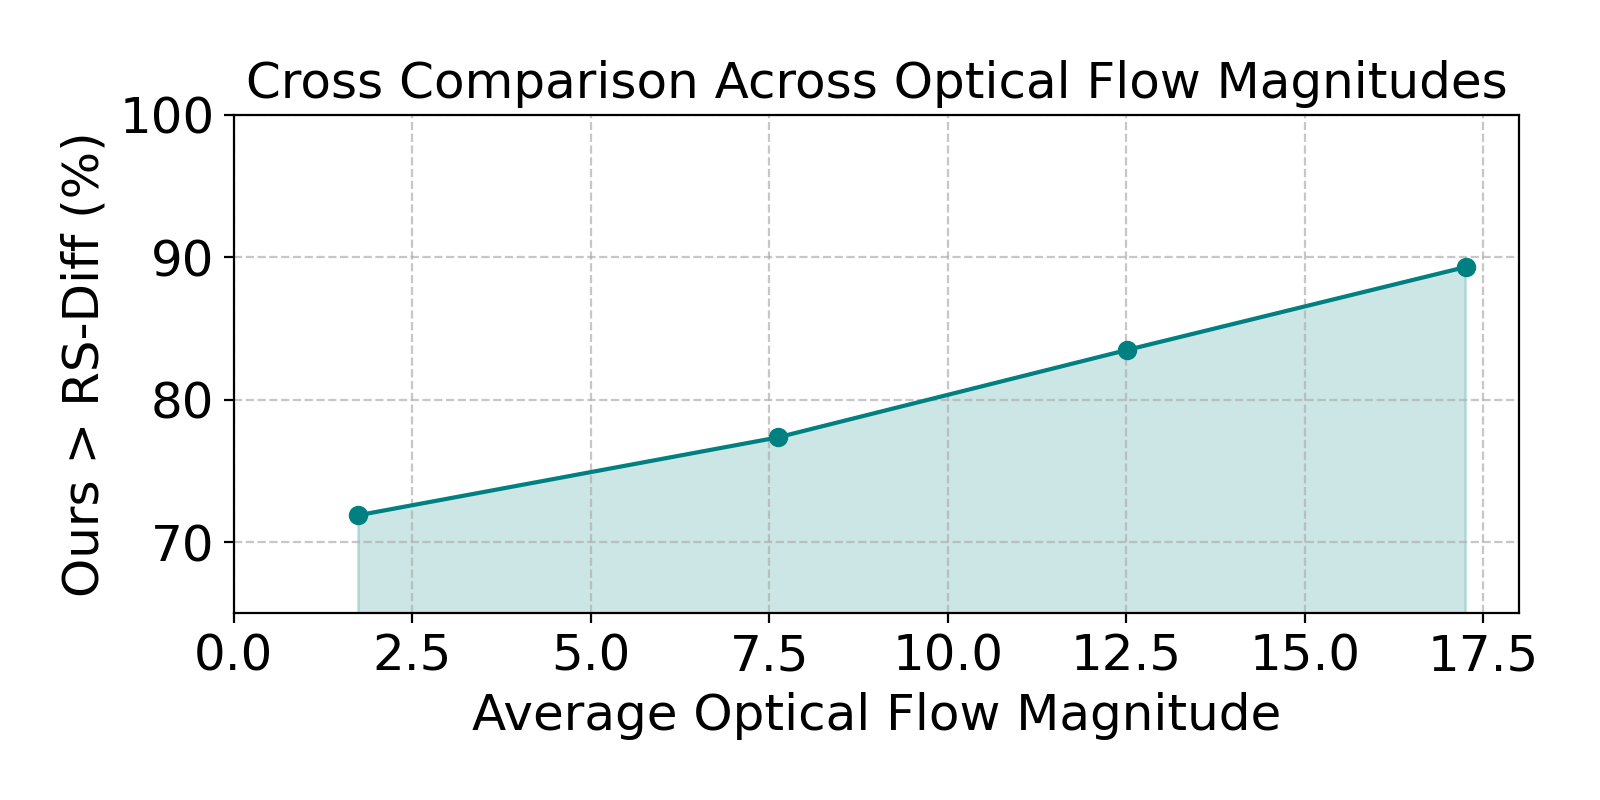
\includegraphics[width=0.9\columnwidth, trim={0cm 0.5cm 0cm 1.5cm}]{collage/psnr_bin_line_vs_flow_zoomed.png}%
    % \vspace{-2mm}
    \caption{Relative performance of our model vs. RS-Diffusion across optical flow magnitudes. Each bin represents the percentage of images where our model achieves higher PSNR.}
    \label{fig:flow_vs_perf}
    \vspace{-1mm}
\end{figure}


\begin{figure}[b!]
    \vspace{-3mm}
    \centering
    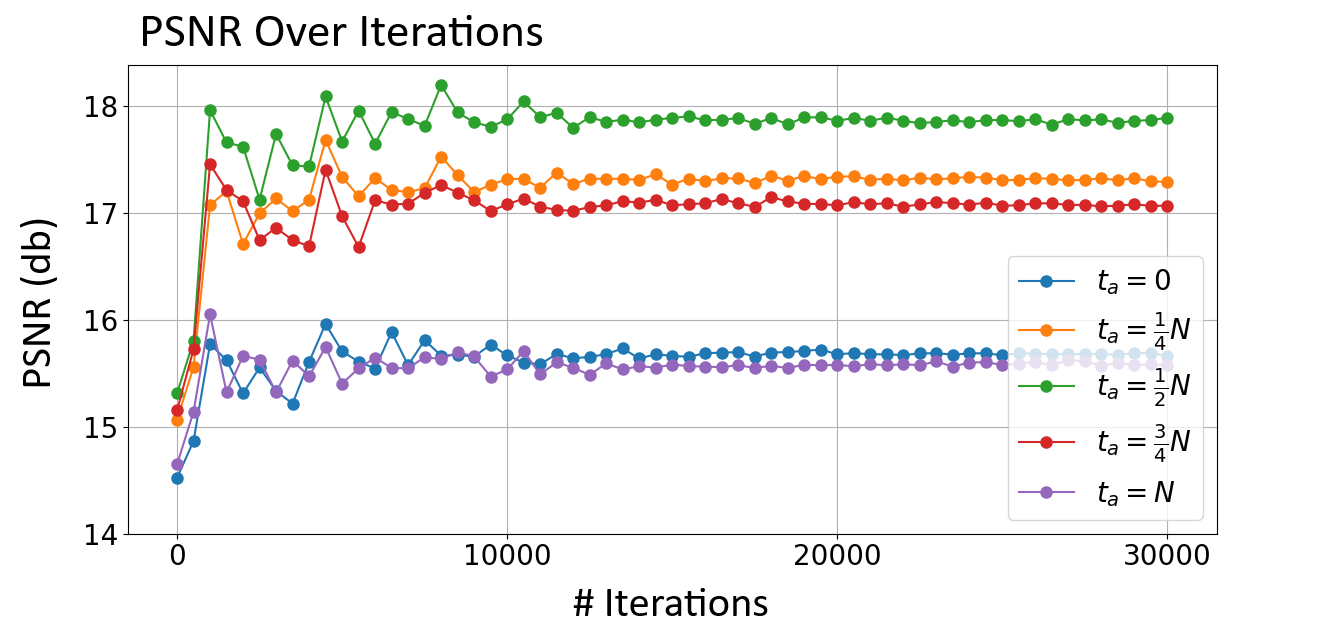
\includegraphics[width=0.49\textwidth, trim=0 2 0 16.5mm,  % left bottom right top
        clip]{X4K_data/figure (1).png} % Path to your first image
    
    \caption{Comparison of PSNR in the five models described in Sec. V-B. Performing a grid search on the possible anchor point location yielded different networks with varying accuracies. These experiments support the use of the anchor point $\frac{N}{2}$ for the real-world scenes.}

    % Comparison of PSNR in the five models described in Sect. 5.B. Each model, with a different anchor point, is represented by a different color on the graph. We validated our theory for anchor points for general scenes. Performing a grid search on the possible anchor point location yielded different networks with varying accuracies. This experiments supported the use of the anchor point $\frac{N}{2}$ for the real-world scenes.
    \vspace{-2mm}
    \label{fig:PSNR_X4K}
\end{figure}









\begin{table}[t!]
\vspace{1mm}
  \caption{Comparisons of anchor points with the first stage of our architecture on \textbf{SYN2} and \textbf{REAL}. These comparisons were conducted on the intermediate RGB images, and $t_a = \frac{N}{2}$ consistently achieves the best or comparable performance.}
  \centering
  \begin{tabular}{c c c c c}
    \hline
    \multirow{2}{*}{Anchor} & \multicolumn{2}{c}{X4K} & \multicolumn{2}{c}{Collocated} \\
    & PSNR & SSIM & PSNR & SSIM \\
    \hline
    $t_a=0$ & 15.594 & 0.578 & 20.238 & 0.639 \\
    $t_a=\frac{N}{4}$ & 17.291 & \textbf{0.630} & 20.292 & 0.640 \\
    $t_a=\frac{N}{2}$ & \textbf{17.733} & 0.629 & \textbf{21.778} & \textbf{0.674} \\
    \hline
  \end{tabular}
  \label{table:AnchorPoint_multi}
  \vspace{-4mm}
\end{table}




\subsection{Ablation Study: Model Configuration}
We evaluated three configurations: \textbf{one-stage}, \textbf{parallel two-stage}, and \textbf{orthogonal two-stage} (Table~\ref{table:collocated_orthogonal_table}). 
\textbf{One-stage} models (Marigold~\cite{StableDiffusion}, Depth-Anything~\cite{DepthAnything}, EcoDepth~\cite{ecodepth}) jointly learn de-rolling and depth but struggle with structural consistency. \textbf{Parallel two-stage} models decouple the tasks sequentially using identical architectures; this improves stability but provides limited gains. 
\textbf{Orthogonal two-stage} models combine distinct architectures (Marigold U-Net for de-rolling and Depth-Anything-V2 for depth) and achieve the highest PSNR, SSIM, AbsRel, and $\delta_1$. Even untuned orthogonal baselines outperform parallel two-stage designs, indicating that sequential specialization of tasks is a pivotal factor behind performance improvements. Fine-tuning further improves results, confirming that the pipeline effectively leverages VFMs for RSC and Monocular Depth Estimation.

\draft{The effects of anchor-point selection and architecture choice were studied independently. Table II isolates anchor-point selection while holding the underlying network architecture fixed. Table III evaluates different architectural configurations while using the optimal anchor point identified in Table II. The results indicate that both factors contribute to performance. Anchor-point selection consistently improves photometric reconstruction quality, while architectural specialization further improves downstream depth estimation metrics.}

% \draft{Because depth estimation is applied to the output of the RS correction stage, and because improvements in PSNR/SSIM consistently correlated with improvements in AbsRel and $\delta1$ throughout our experiments, we performed anchor-point ablations using the intermediate RGB reconstruction metrics. This isolates the effect of anchor-point selection while avoiding confounding effects from retraining multiple downstream depth networks.}


\subsection{Ablation Study: Anchor Points in Other RSC Algorithms}
We evaluated RS-Diffusion~\cite{RS-Diffusion} across a sweep of anchor points and found that centering the predicted flow at the temporal midpoint ($t_{\text{anch}} = \frac{N}{2}$) consistently yields the best reconstruction on synthetic and real RS images. \draft{RS-Diffusion was chosen for ablation due to its ability to change predicted flow easily without retraining.} This confirms that mid-exposure alignment improves performance across different RSC methods without retraining, highlighting the generality of the anchor-point insight (Fig. \ref{fig:teaser_results}).



\begin{table}[t!]
    \centering
    \caption{Depth estimation performance in a legged robot scenario comparing the rolling shutter depth against our method. AbsRel and $\delta_1$ are averaged over $1500$ images collected across three outdoor locations.}
    \setlength{\tabcolsep}{12pt}
    \renewcommand{\arraystretch}{1.2}
    \begin{tabular}{lcc}
        \toprule
        Method & absRel $\downarrow$ & $\delta_1 \uparrow$ \\
        \midrule
        Raw RS Image & 0.112 & 0.895 \\
        Our Algorithm & \textbf{0.096} & \textbf{0.903} \\
        \bottomrule
    \end{tabular}

    \label{tab:puppy_pi}
\end{table}




\subsection{Effectiveness on Legged Robots}

% Legged robots are subject to rapid and irregular motion. Because RS cameras expose image rows sequentially, abrupt accelerations and rotations induce geometric warping that degrades depth estimation. As shown in Fig.~\ref{Fig:puppy_pi_qual}, the RS depth maps exhibit visible distortions that can negatively impact downstream perception and planning.

To evaluate our method in this real-world setting, we collected $1500$ images across three outdoor locations using the collocated sensor system mounted on Puppy-Pi. Runtime measurements were performed on an NVIDIA RTX A6000 GPU using FP16 inference at a resolution of $300\times300$. To improve deployment efficiency, the diffusion model was accelerated by reducing the number of denoising steps from $50$ to $10$, reducing the average inference time from $2850$~ms to $349$~ms.

As shown in Table~\ref{tab:puppy_pi}, our method reduces AbsRel by $14.3\%$ and improves $\delta_1$ accuracy by $0.9\%$ over raw RS input without additional fine-tuning beyond training on the REAL dataset. The qualitative results in Fig.~\ref{Fig:puppy_pi_qual} are consistent with these improvements, where rolling shutter--induced warping is visibly mitigated. While the proposed pipeline demonstrates promising low-latency performance, deployment at higher image resolutions or alongside additional perception tasks presents a natural computational trade-off due to increased diffusion and image-processing costs. Improving scalability through more efficient diffusion strategies, model compression, or shared-backbone architectures remains an important direction for future work.

% \begin{figure}[h!]
%     \centering

%     % =======================
%     % Top row: diagram + single example column
%     % =======================
%     \begin{minipage}{0.95\linewidth}
%         \centering
%         % Combined diagram and example
%         \begin{minipage}{0.5\linewidth}
%             \centering
%             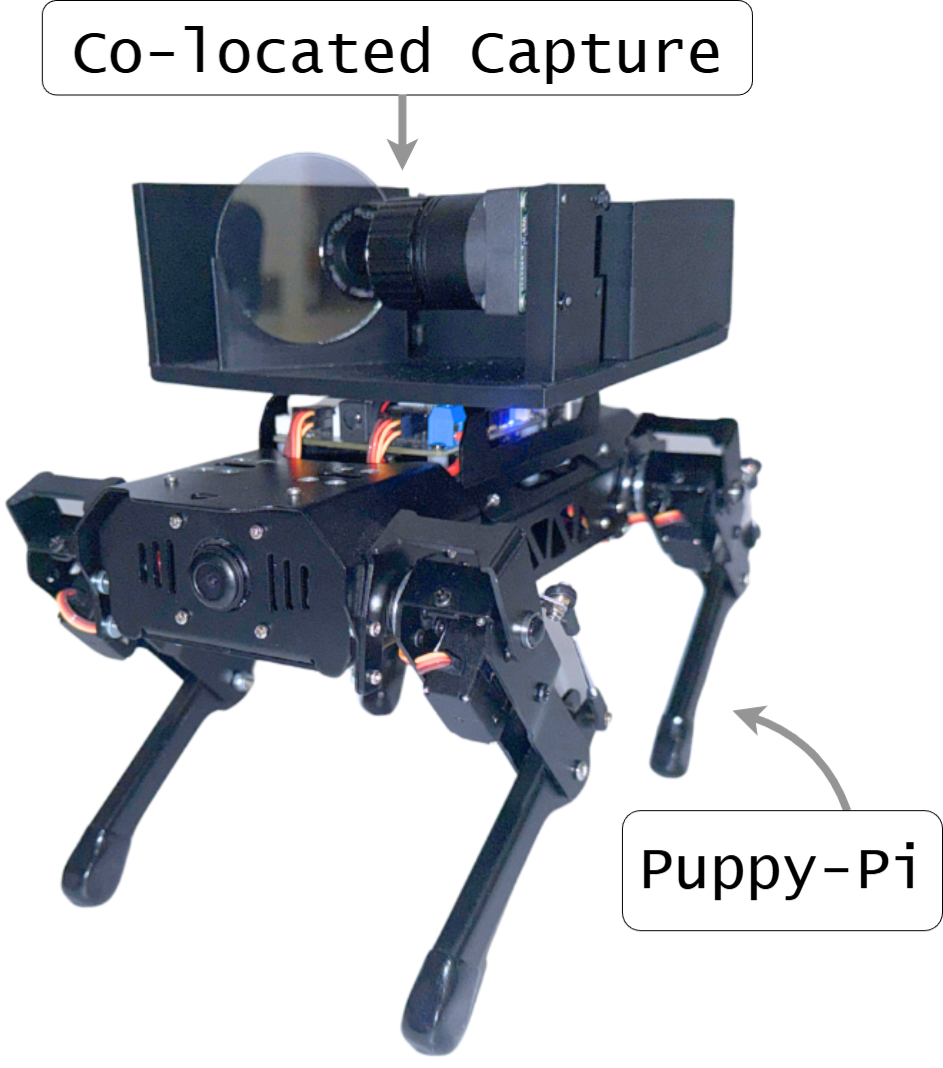
\includegraphics[width=\linewidth]{Figures/puppy-pi.drawio.png}
%         \end{minipage}%
%         \hspace{1mm}
%         \begin{minipage}{0.25\linewidth}
%             \centering
%             % Example column: Input / Prediction / Ground Truth
%             % Row 1 — Input
%             \begin{minipage}{0.2\linewidth}
%                 \centering
%                 \rotatebox{90}{\small Input}
%             \end{minipage}%
%             \begin{minipage}{0.75\linewidth}
%                 \centering
%                 
\includegraphics[width=\textwidth]{puppy-pi/rs/frame55.png}
%             \end{minipage}

%             \vspace{1mm}

%             % Row 2 — Prediction
%             \begin{minipage}{0.2\linewidth}
%                 \centering
%                 \rotatebox{90}{\small Prediction}
%             \end{minipage}%
%             \begin{minipage}{0.75\linewidth}
%                 \centering
%                 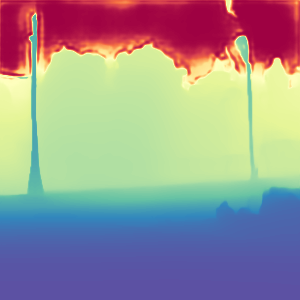
\includegraphics[width=\textwidth]{puppy-pi/depth/rs/frame55_pred.png}
%             \end{minipage}

%             \vspace{1mm}

%             % Row 3 — Ground Truth
%             \begin{minipage}{0.2\linewidth}
%                 \centering
%                 \rotatebox{90}{\small Ground Truth}
%             \end{minipage}%
%             \begin{minipage}{0.75\linewidth}
%                 \centering
%                 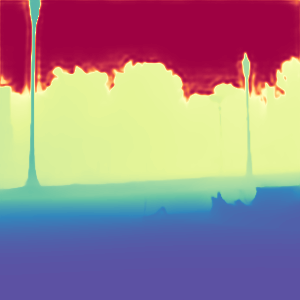
\includegraphics[width=\textwidth]{puppy-pi/depth/gs/frame55.png}
%             \end{minipage}
%         \end{minipage}
%     \end{minipage}

%     \vspace{2mm}

%     % =======================
%     % Bottom: Table
%     % =======================
%     \begin{minipage}{0.65\linewidth}
%         \centering
%         \begin{tabular}{lcc}
%             \toprule
%             Method & absRel $\downarrow$ & $\delta 1 \uparrow$ \\
%             \midrule
%             Raw RS Image & 0.1119 & 0.8958 \\
%             Our Algorithm & \textbf{0.0963} & \textbf{0.9033} \\
%             \bottomrule
%         \end{tabular}
%     \end{minipage}

%     \caption{Left: schematic illustration of the RS effect on the Puppy-Pi. Right: input, prediction, and ground truth for a single frame. Bottom: dataset-averaged depth metrics comparing raw RS input and corrected output. 
%     %\JI{What does this image/result mean...please revise @Vaishnav }
%     }
%     \label{fig:puppy}
% \end{figure}

\begin{figure}[t]
\centering
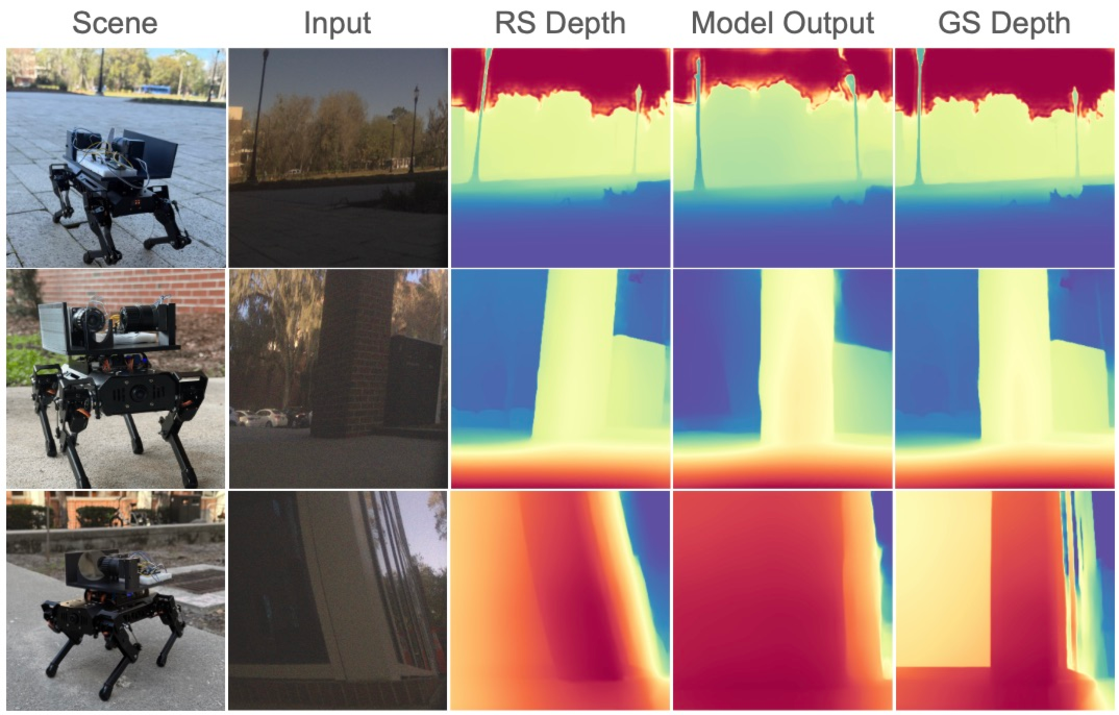
\includegraphics[width=0.49\textwidth]{Figures/puppy_pi_exp_short.pdf}
\caption{Visualizations of our model for RS distortions in legged robots. The qualitative results demonstrate effective rectification of rolling shutter artifacts in legged robotic scenarios.}
\label{Fig:puppy_pi_qual}
\vspace{-3mm}
\end{figure}

%mention number of images/ Scene where rolling shutter is more pronounced, Add rolling shutter output in  image.
% To validate the applicability of our method to mobile robotics, a test dataset was captured with the co-located system attached to Puppy-Pi. The model, using the same weights as the one trained on the co-located dataset, was modified through floating-point changes (32 to 16) and denoise steps (50 to 10) to drastically reduce runtime. These changes reduce average runtime on the pipeline from 2850ms to 349ms, providing a close to real time pipeline for inference. Highlighted visualizations and metrics from data captured on puppy-pi and model output can be seen in Fig. \ref{fig:puppy}.
% \subsection{Ablation Study: Anchor Points}

% Finally, we evaluated the impact of anchor points across synthetic (\textbf{SYN2}) and real-world (\textbf{REAL}) datasets. For SYN2, we trained models with anchor points $t_a = 0, \frac{1}{4}N, \frac{1}{2}N, \frac{3}{4}N, N$, using identical RS inputs. PSNR and SSIM consistently improved as the anchor approached the midpoint, confirming the theoretical prediction (Fig.~\ref{fig:PSNR_X4K}).  

% In REAL, each anchor corresponds to a distinct capture, introducing natural variation. Models trained near the temporal midpoint again achieved higher PSNR and SSIM, demonstrating that the anchor-point formulation generalizes to real-world scenes. These results emphasize the importance of temporal alignment in RS-GS correction, independent of the specific architectures used.

% \noindent \textbf{Effect of Anchor Point on RS-Diffusion.} 


%\JI{What did we learn and where are the closing paragraph}


% \JI{Missing conclusion section}
\section{Conclusion}
In this paper, we investigate monocular depth estimation under severe rolling shutter distortions induced by robot ego-motion and identify anchor-point selection as a key factor governing geometric consistency and depth accuracy. By explicitly modeling this temporal reference, we demonstrate that existing rolling shutter correction methods and vision foundation models can be substantially improved without architectural modifications or retraining. Using a new collocated RS-GS dataset and extensive synthetic and real-world experiments, we demonstrated robust depth estimation under large distortions and aggressive motion, including deployment on a legged robot with an inference latency under $400$\,ms. These findings highlight the importance of temporal alignment in rolling shutter perception and suggest that anchor-based modeling can serve as a simple yet effective design principle for improving visual perception in mobile robotic systems.

\section*{Acknowledgments}
The authors thank Amazon Robotics for their support of this work with AGR DTD 10-06-2025. We also thank the National Science Foundation and the Office of Naval Research for their support. The authors were partially supported by NSF grants 1942444 and 2330416 as well as ONR grants N000142312429 and N000142312363.
% We thank the National Science Foundation and the Office of Naval Research for their support and the authors were partially supported by NSF grants 1942444 and 2330416 as well as ONR grants N000142312429 and N000142312363.












\bibliographystyle{IEEEtran}
\bibliography{main}

\end{document}
